%%%%%%%%%%%%%%%%%%%%%%%%%%%%%%%%%%%%%%%%%%%%%%%%%%%%%%%%%%%%%%%%%%%%%%
% Template for a UBC-compliant dissertation
% At the minimum, you will need to change the information found
% after the "Document meta-data"
% see https://github.com/briandealwis/ubcdiss
%
%!TEX TS-program = pdflatex
%!TEX encoding = UTF-8 Unicode

%% The ubcdiss class provides several options:
%%   gpscopy (aka fogscopy)
%%       set parameters to exactly how GPS specifies
%%         * single-sided
%%         * page-numbering starts from title page
%%         * the lists of figures and tables have each entry prefixed
%%           with 'Figure' or 'Table'
%%       This can be tested by `\ifgpscopy ... \else ... \fi'
%%   10pt, 11pt, 12pt
%%       set default font size
%%   oneside, twoside
%%       whether to format for single-sided or double-sided printing
%%   balanced
%%       when double-sided, ensure page content is centred
%%       rather than slightly offset (the default)
%%   singlespacing, onehalfspacing, doublespacing
%%       set default inter-line text spacing; the ubcdiss class
%%       provides \textspacing to revert to this configured spacing
%%   draft
%%       disable more intensive processing, such as including
%%       graphics, etc.
%%

% For submission to GPS
\documentclass[gpscopy,onehalfspacing,11pt]{ubcdiss}

% Setting to Kiefl's Margin requests
\usepackage{geometry}
\geometry{lmargin=2.7cm, rmargin=2.4cm}

% For your own copies (looks nicer)
% \documentclass[balanced,twoside,11pt]{ubcdiss}

%%%%%%%%%%%%%%%%%%%%%%%%%%%%%%%%%%%%%%%%%%%%%%%%%%%%%%%%%%%%%%%%%%%%%%
%%%%%%%%%%%%%%%%%%%%%%%%%%%%%%%%%%%%%%%%%%%%%%%%%%%%%%%%%%%%%%%%%%%%%%
%%
%% FONTS:
%% 
%% The defaults below configures Times Roman for the serif font,
%% Helvetica for the sans serif font, and Courier for the
%% typewriter-style font.  Configuring fonts can be time
%% consuming; we recommend skipping to END FONTS!
%% 
%% If you're feeling brave, have lots of time, and wish to use one
%% your platform's native fonts, see the commented out bits below for
%% XeTeX/XeLaTeX.  This is not for the faint at heart. 
%% (And shouldn't you be writing? :-)
%%

%% NFSS font specification (New Font Selection Scheme)
\usepackage{times,mathptmx,courier}
\usepackage[scaled=1]{helvet}

%% Math or theory people may want to include the handy AMS macros
\usepackage{amssymb}
\usepackage{amsmath}
\usepackage{amsfonts}
\usepackage{siunitx}

%% The pifont package provides access to the elements in the dingbat font.   
%% Use \ding{##} for a particular dingbat (see p7 of psnfss2e.pdf)
%%   Useful:
%%     51,52 different forms of a checkmark
%%     54,55,56 different forms of a cross (saltyre)
%%     172-181 are 1-10 in open circle (serif)
%%     182-191 are 1-10 black circle (serif)
%%     192-201 are 1-10 in open circle (sans serif)
%%     202-211 are 1-10 in black circle (sans serif)
%% \begin{dinglist}{##}\item... or dingautolist (which auto-increments)
%% to create a bullet list with the provided character.
\usepackage{pifont}

%%%%%%%%%%%%%%%%%%%%%%%%%%%%%%%%%%%%%%%%%%%%%%%%%%%%%%%%%%%%%%%%%%%%%%
%% Configure fonts for XeTeX / XeLaTeX using the fontspec package.
%% Be sure to check out the fontspec documentation.
%\usepackage{fontspec,xltxtra,xunicode}	% required
%\defaultfontfeatures{Mapping=tex-text}	% recommended
%% Minion Pro and Myriad Pro are shipped with some versions of
%% Adobe Reader.  Adobe representatives have commented that these
%% fonts can be used outside of Adobe Reader.
%\setromanfont[Numbers=OldStyle]{Minion Pro}
%\setsansfont[Numbers=OldStyle,Scale=MatchLowercase]{Myriad Pro}
%\setmonofont[Scale=MatchLowercase]{Andale Mono}

%% Other alternatives:
%\setromanfont[Mapping=tex-text]{Adobe Caslon}
%\setsansfont[Scale=MatchLowercase]{Gill Sans}
%\setsansfont[Scale=MatchLowercase,Mapping=tex-text]{Futura}
%\setmonofont[Scale=MatchLowercase]{Andale Mono}
%\newfontfamily{\SYM}[Scale=0.9]{Zapf Dingbats}
%% END FONTS
%%%%%%%%%%%%%%%%%%%%%%%%%%%%%%%%%%%%%%%%%%%%%%%%%%%%%%%%%%%%%%%%%%%%%%
%%%%%%%%%%%%%%%%%%%%%%%%%%%%%%%%%%%%%%%%%%%%%%%%%%%%%%%%%%%%%%%%%%%%%%



%%%%%%%%%%%%%%%%%%%%%%%%%%%%%%%%%%%%%%%%%%%%%%%%%%%%%%%%%%%%%%%%%%%%%%
%%%%%%%%%%%%%%%%%%%%%%%%%%%%%%%%%%%%%%%%%%%%%%%%%%%%%%%%%%%%%%%%%%%%%%
%%
%% Recommended packages
%%
\usepackage{checkend}	% better error messages on left-open environments
\usepackage{graphicx}	% for incorporating external images

%% booktabs: provides some special commands for typesetting tables as used
%% in excellent journals.  Ignore the examples in the Lamport book!
\usepackage{booktabs}

%% listings: useful support for including source code listings, with
%% optional special keyword formatting.  The \lstset{} causes
%% the text to be typeset in a smaller sans serif font, with
%% proportional spacing.
\usepackage{listings}
\lstset{basicstyle=\sffamily\scriptsize,showstringspaces=false,fontadjust}

%% The acronym package provides support for defining acronyms, providing
%% their expansion when first used, and building glossaries.  See the
%% example in glossary.tex and the example usage throughout the example
%% document.
%% NOTE: to use \MakeTextLowercase in the \acsfont command below,
%%   we *must* use the `nohyperlinks' option -- it causes errors with
%%   hyperref otherwise.  See Section 5.2 in the ``LaTeX 2e for Class
%%   and Package Writers Guide'' (clsguide.pdf) for details.
\usepackage[nohyperlinks]{acronym}
%% The ubcdiss.cls loads the `textcase' package which provides commands
%% for upper-casing and lower-casing text.  The following causes
%% the acronym package to typeset acronyms in small-caps
%% as recommended by Bringhurst.
%\renewcommand{\acsfont}[1]{{\scshape \MakeTextLowercase{#1}}}

%% color: add support for expressing colour models.  Grey can be used
%% to great effect to emphasize other parts of a graphic or text.
%% For an excellent set of examples, see Tufte's "Visual Display of
%% Quantitative Information" or "Envisioning Information".
\usepackage{color}
\definecolor{greytext}{gray}{0.5}

%% comment: provides a new {comment} environment: all text inside the
%% environment is ignored.
%%   \begin{comment} ignored text ... \end{comment}
\usepackage{comment}

%% The natbib package provides more sophisticated citing commands
%% such as \citeauthor{} to provide the author names of a work,
%% \citet{} to produce an author-and-reference citation,
%% \citep{} to produce a parenthetical citation.
%% We use \citeeg{} to provide examples
\usepackage[numbers,sort&compress]{natbib}
\newcommand{\citeeg}[1]{\citep[e.g.,][]{#1}}

%% The titlesec package provides commands to vary how chapter and
%% section titles are typeset.  The following uses more compact
%% spacings above and below the title.  The titleformat that follow
%% ensure chapter/section titles are set in singlespace.
\usepackage[compact]{titlesec}
\titleformat*{\section}{\singlespacing\raggedright\bfseries\Large}
\titleformat*{\subsection}{\singlespacing\raggedright\bfseries\large}
\titleformat*{\subsubsection}{\singlespacing\raggedright\bfseries}
\titleformat*{\paragraph}{\singlespacing\raggedright\itshape}

%% The caption package provides support for varying how table and
%% figure captions are typeset.
\usepackage[format=hang,indention=-1cm,labelfont={bf},margin=1em]{caption}

%% url: for typesetting URLs and smart(er) hyphenation.
%% \url{http://...} 
\usepackage{url}
\urlstyle{sf}	% typeset urls in sans-serif


%%%%%%%%%%%%%%%%%%%%%%%%%%%%%%%%%%%%%%%%%%%%%%%%%%%%%%%%%%%%%%%%%%%%%%
%%%%%%%%%%%%%%%%%%%%%%%%%%%%%%%%%%%%%%%%%%%%%%%%%%%%%%%%%%%%%%%%%%%%%%
%%
%% Possibly useful packages: you may need to explicitly install
%% these from CTAN if they aren't part of your distribution;
%% teTeX seems to ship with a smaller base than MikTeX and MacTeX.
%%
%\usepackage{pdfpages}	% insert pages from other PDF files
%\usepackage{longtable}	% provide tables spanning multiple pages
%\usepackage{chngpage}	% support changing the page widths on demand
%\usepackage{tabularx}	% an enhanced tabular environment

%% enumitem: support pausing and resuming enumerate environments.
%\usepackage{enumitem}

%% rotating: provides two environments, sidewaystable and sidewaysfigure,
%% for typesetting tables and figures in landscape mode.  
%\usepackage{rotating}

%% subfig: provides for including subfigures within a figure,
%% and includes being able to separately reference the subfigures.
%\usepackage{subfig}

%% ragged2e: provides several new new commands \Centering, \RaggedLeft,
%% \RaggedRight and \justifying and new environments Center, FlushLeft,
%% FlushRight and justify, which set ragged text and are easily
%% configurable to allow hyphenation.
% \usepackage{ragged2e}
% \raggedright
% \hyphenpenalty=10000

%% The ulem package provides a \sout{} for striking out text and
%% \xout for crossing out text.  The normalem and normalbf are
%% necessary as the package messes with the emphasis and bold fonts
%% otherwise.
%\usepackage[normalem,normalbf]{ulem}    % for \sout

%%%%%%%%%%%%%%%%%%%%%%%%%%%%%%%%%%%%%%%%%%%%%%%%%%%%%%%%%%%%%%%%%%%%%%
%% HYPERREF:
%% The hyperref package provides for embedding hyperlinks into your
%% document.  By default the table of contents, references, citations,
%% and footnotes are hyperlinked.
%%
%% Hyperref provides a very handy command for doing cross-references:
%% \autoref{}.  This is similar to \ref{} and \pageref{} except that
%% it automagically puts in the *type* of reference.  For example,
%% referencing a figure's label will put the text `Figure 3.4'.
%% And the text will be hyperlinked to the appropriate place in the
%% document.
%%
%% Generally hyperref should appear after most other packages

%% The following puts hyperlinks in very faint grey boxes.
%% The `pagebackref' causes the references in the bibliography to have
%% back-references to the citing page; `backref' puts the citing section
%% number.  See further below for other examples of using hyperref.
%% 2009/12/09: now use `linktocpage' (Jacek Kisynski): GPS now prefers
%%   that the ToC, LoF, LoT place the hyperlink on the page number,
%%   rather than the entry text.
\usepackage[bookmarks,bookmarksnumbered,%
    allbordercolors={0.8 0.8 0.8},%
    pagebackref,linktocpage%
    ]{hyperref}
    
    
\usepackage{color,soul}
%% The following change how the the back-references text is typeset in a
%% bibliography when `backref' or `pagebackref' are used
%%
%% Change \nocitations if you'd like some text shown where there
%% are no citations found (e.g., pulled in with \nocite{xxx})
\newcommand{\nocitations}{\relax}
%%\newcommand{\nocitations}{No citations}
%%
%\renewcommand*{\backref}[1]{}% necessary for backref < 1.33
\renewcommand*{\backrefsep}{,~}%
\renewcommand*{\backreftwosep}{,~}% ', and~'
\renewcommand*{\backreflastsep}{,~}% ' and~'
\renewcommand*{\backrefalt}[4]{%
\textcolor{greytext}{\ifcase #1%
\nocitations%
\or
\(\rightarrow\) page #2%
\else
\(\rightarrow\) pages #2%
\fi}}


%% The following uses most defaults, which causes hyperlinks to be
%% surrounded by colourful boxes; the colours are only visible in
%% PDFs and don't show up when printed:
%\usepackage[bookmarks,bookmarksnumbered]{hyperref}

%% The following disables the colourful boxes around hyperlinks.
%\usepackage[bookmarks,bookmarksnumbered,pdfborder={0 0 0}]{hyperref}

%% The following disables all hyperlinking, but still enabled use of
%% \autoref{}
%\usepackage[draft]{hyperref}

%% The following commands causes chapter and section references to
%% uppercase the part name.
\renewcommand{\chapterautorefname}{Chapter}
\renewcommand{\sectionautorefname}{Section}
\renewcommand{\subsectionautorefname}{Section}
\renewcommand{\subsubsectionautorefname}{Section}

%% If you have long page numbers (e.g., roman numbers in the 
%% preliminary pages for page 28 = xxviii), you might need to
%% uncomment the following and tweak the \@pnumwidth length
%% (default: 1.55em).  See the tocloft documentation at
%% http://www.ctan.org/tex-archive/macros/latex/contrib/tocloft/
% \makeatletter
% \renewcommand{\@pnumwidth}{3em}
% \makeatother

%%%%%%%%%%%%%%%%%%%%%%%%%%%%%%%%%%%%%%%%%%%%%%%%%%%%%%%%%%%%%%%%%%%%%%
%%%%%%%%%%%%%%%%%%%%%%%%%%%%%%%%%%%%%%%%%%%%%%%%%%%%%%%%%%%%%%%%%%%%%%
%%
%% Some special settings that controls how text is typeset
%%
% \raggedbottom		% pages don't have to line up nicely on the last line
% \sloppy		% be a bit more relaxed in inter-word spacing
\clubpenalty=10000	% try harder to avoid orphans
\widowpenalty=10000	% try harder to avoid widows
% \tolerance=1000

%% And include some of our own useful macros
% This file provides examples of some useful macros for typesetting
% dissertations.  None of the macros defined here are necessary beyond
% for the template documentation, so feel free to change, remove, and add
% your own definitions.
%
% We recommend that you define macros to separate the semantics
% of the things you write from how they are presented.  For example,
% you'll see definitions below for a macro \file{}: by using
% \file{} consistently in the text, we can change how filenames
% are typeset simply by changing the definition of \file{} in
% this file.
% 
%% The following is a directive for TeXShop to indicate the main file
%%!TEX root = diss.tex

\newcommand{\NA}{\textsc{n/a}}	% for "not applicable"
\newcommand{\eg}{e.g.,\ }	% proper form of examples (\eg a, b, c)
\newcommand{\ie}{i.e.,\ }	% proper form for that is (\ie a, b, c)
\newcommand{\etal}{\emph{et al}}

% Some useful macros for typesetting terms.
\newcommand{\file}[1]{\texttt{#1}}
\newcommand{\class}[1]{\texttt{#1}}
\newcommand{\latexpackage}[1]{\href{http://www.ctan.org/macros/latex/contrib/#1}{\texttt{#1}}}
\newcommand{\latexmiscpackage}[1]{\href{http://www.ctan.org/macros/latex/contrib/misc/#1.sty}{\texttt{#1}}}
\newcommand{\env}[1]{\texttt{#1}}
\newcommand{\BibTeX}{Bib\TeX}

% Define a command \doi{} to typeset a digital object identifier (DOI).
% Note: if the following definition raise an error, then you likely
% have an ancient version of url.sty.  Either find a more recent version
% (3.1 or later work fine) and simply copy it into this directory,  or
% comment out the following two lines and uncomment the third.
\DeclareUrlCommand\DOI{}
\newcommand{\doi}[1]{\href{http://dx.doi.org/#1}{\DOI{doi:#1}}}
%\newcommand{\doi}[1]{\href{http://dx.doi.org/#1}{doi:#1}}

% Useful macro to reference an online document with a hyperlink
% as well with the URL explicitly listed in a footnote
% #1: the URL
% #2: the anchoring text
\newcommand{\webref}[2]{\href{#1}{#2}\footnote{\url{#1}}}

% epigraph is a nice environment for typesetting quotations
\makeatletter
\newenvironment{epigraph}{%
	\begin{flushright}
	\begin{minipage}{\columnwidth-0.75in}
	\begin{flushright}
	\@ifundefined{singlespacing}{}{\singlespacing}%
    }{
	\end{flushright}
	\end{minipage}
	\end{flushright}}
\makeatother

% \FIXME{} is a useful macro for noting things needing to be changed.
% The following definition will also output a warning to the console
\newcommand{\FIXME}[1]{\typeout{**FIXME** #1}\textbf{[FIXME: #1]}}

% END


%%%%%%%%%%%%%%%%%%%%%%%%%%%%%%%%%%%%%%%%%%%%%%%%%%%%%%%%%%%%%%%%%%%%%%
%%%%%%%%%%%%%%%%%%%%%%%%%%%%%%%%%%%%%%%%%%%%%%%%%%%%%%%%%%%%%%%%%%%%%%
%%
%% Things that I (Jonah) have added.
%%
\setlength\arrayrulewidth{1.2pt} % thicker table lines
\def\arraystretch{1.5} % stretches table spacing 
\usepackage{rotating} % allows the command \sidewaystable to be used
\usepackage{lmodern,bm} % adds the \bm command for italic bold math
\renewcommand{\thefootnote}{\fnsymbol{footnote}} % changes footnote numbering to symbolic



\usepackage{nottocite}

%%%%%%%%%%%%%%%%%%%%%%%%%%%%%%%%%%%%%%%%%%%%%%%%%%%%%%%%%%%%%%%%%%%%%%
%%%%%%%%%%%%%%%%%%%%%%%%%%%%%%%%%%%%%%%%%%%%%%%%%%%%%%%%%%%%%%%%%%%%%%

%%
%% Document meta-data: be sure to also change the \hypersetup information
%%

\title{Measurement of the $2^+_2 \rightarrow 2^+_1$ Electric Monopole Transition Strength in $^{110}$Pd for the Study of Nuclear Structure}
%\subtitle{If you want a subtitle}

\author{Jonah Berean-Dutcher}
% \previousdegree{B. Basket Weaving, University of Illustrious Arts, 1991}
% \previousdegree{M. Silly Walks, Another University, 1994}

% What is this dissertation for?
\degreetitle{Bachelor of Science}

\institution{The University of British Columbia}
\campus{Vancouver}

\faculty{The Faculty of Science}
\department{Honours Physics}
\submissionmonth{April}
\submissionyear{2018}

%% hyperref package provides support for embedding meta-data in .PDF
%% files
\hypersetup{
  pdftitle={Change this title!  (DRAFT: \today)},
  pdfauthor={Johnny Canuck},
  pdfkeywords={Your keywords here}
}


%%%%%%%%%%%%%%%%%%%%%%%%%%%%%%%%%%%%%%%%%%%%%%%%%%%%%%%%%%%%%%%%%%%%%%
%%%%%%%%%%%%%%%%%%%%%%%%%%%%%%%%%%%%%%%%%%%%%%%%%%%%%%%%%%%%%%%%%%%%%%
%% 
%% The document content
%%

%% LaTeX's \includeonly commands causes any uses of \include{} to only
%% include files that are in the list.  This is helpful to produce
%% subsets of your thesis (e.g., for committee members who want to see
%% the dissertation chapter by chapter).  It also saves time by 
%% avoiding reprocessing the entire file.
%\includeonly{intro,conclusions}
%\includeonly{discussion}



\begin{document}

%%%%%%%%%%%%%%%%%%%%%%%%%%%%%%%%%%%%%%%%%%%%%%%%%%%%%%%%%%%%%%%%%%%%%%
%%%%%%%%%%%%%%%%%%%%%%%%%%%%%%%%%%%%%%%%%%%%%%%%%%%%%%%%%%%%%%%%%%%%%%
%%
%% Useful commands
%%
\newcommand{\pd}{$^{110}\mathrm{Pd}$ }
\newcommand{\gr}{$\gamma$-ray }
\newcommand{\ro}{$\rho^2(E0)$ }


%%%%%%%%%%%%%%%%%%%%%%%%%%%%%%%%%%%%%%%%%%%%%%%%%%%%%%%%%%%%%%%%%%%%%%
%%%%%%%%%%%%%%%%%%%%%%%%%%%%%%%%%%%%%%%%%%%%%%%%%%%%%%%%%%%%%%%%%%%%%%

%%%%%%%%%%%%%%%%%%%%%%%%%%%%%%%%%%%%%%%%%%%%%%%%%%
%% From Thesis Components: Tradtional Thesis
%% <http://www.grad.ubc.ca/current-students/dissertation-thesis-preparation/order-components>

% Preliminary Pages (numbered in lower case Roman numerals)
%    1. Title page (mandatory)
\maketitle

%    2. Abstract (mandatory - maximum 350 words)
%% The following is a directive for TeXShop to indicate the main file
%%!TEX root = diss.tex

\chapter{Abstract}

A measurement of the strength of the $E0$ transition between the $2_2^+$ and $2_1^+$ states of the nucleus $^{110}\mathrm{Pd}$ was performed. $E0$ transition strength measurements serve as a sensitive probe of the degree of nuclear shape mixing between different intrinsic structures within nuclei. Analysis was conducted of spectroscopic $\gamma$-ray and internal conversion electron data obtained by inelastic scattering of an accelerated alpha particle beam off of a $^{110}\mathrm{Pd}$ target. Internal conversion coefficients were measured for a range of transitions from the nuclei $^{110}\mathrm{Pd}$, $^{109}\mathrm{Pd}$, and $^{111}\mathrm{Ag}$. The $\gamma$-ray data was collected by the TRIUMF-ISAC Gamma-Ray Escape Spectrometer (TIGRESS), and the internal conversion electron data by the Spectrometer for Internal Conversion Electrons (SPICE). The use of these detectors in parallel required a study of the relative detection efficiencies, as a function of particle energy, such that absolute internal conversion coefficient measurements could be justified as accurate. In particular, SPICE was characterized further via a study of simulated particle detection efficiency using the Geant4 simulation toolkit. The resultant internal conversion coefficient measurements were combined with literature half life and branching ratio information to determine the $E0$ transition strength for the first time. A Monte Carlo error analysis approach was used to arrive at a measured limit on the true value of the $E0$ transition strength. This measured limit constitutes an effectively negligible $E0$ transition component, and evidence of little to no shape mixing between the intrinsic structures of the nucleus $^{110}\mathrm{Pd}$.

% Consider placing version information if you circulate multiple drafts
%\vfill
%\begin{center}
%\begin{sf}
%\fbox{Revision: \today}
%\end{sf}
%\end{center} 
\cleardoublepage

%    3. Lay Summary (Effective May 2017, mandatory - maximum 150 words)
%% The following is a directive for TeXShop to indicate the main file
%%!TEX root = diss.tex

%% https://www.grad.ubc.ca/current-students/dissertation-thesis-preparation/preliminary-pages
%% 
%% LAY SUMMARY Effective May 2017, all theses and dissertations must
%% include a lay summary.  The lay or public summary explains the key
%% goals and contributions of the research/scholarly work in terms that
%% can be understood by the general public. It must not exceed 150
%% words in length.

\chapter{Lay Summary}

This nuclear physics research investigates the phenomenon of shape coexistence in atomic nuclei. The ways in which energetic nuclei get rid of excess energy, energy that makes their inhabited physical state an unstable one, can lead to an interpretation of their nuclear shape. The nuclei of different atoms are found in a range of spheroidal shapes, which can be characterized as different deformations of the simple, ball shape, from prolate (like a rugby ball), to oblate (like a lentil), and to yet more exotic configurations. Shape coexistence refers to the unique instance wherein a single nuclei can simultaneously coexist in multiple such shapes, a fundamentally quantum mechanical phenomenon. In this research the data from high-energy nuclear collisions, collected at TRIUMF, Canada's national particle accelerator centre, are analyzed. The conclusions as they pertain to this shape coexistence phenomenon are discussed. \newline


\cleardoublepage

%    4. Preface
%%% The following is a directive for TeXShop to indicate the main file
%%!TEX root = diss.tex

\chapter{Preface}

At \ac{UBC}, a preface may be required.  Be sure to check the
\ac{GPS} guidelines as they may have specific content to be included.

%\cleardoublepage

%    5. Table of contents (mandatory - list all items in the preliminary pages
%    starting with the abstract, followed by chapter headings and
%    subheadings, bibliographies and appendices)
\tableofcontents
\cleardoublepage	% required by tocloft package

%    6. List of tables (mandatory if thesis has tables)
\listoftables
\cleardoublepage	% required by tocloft package

%    7. List of figures (mandatory if thesis has figures)
\listoffigures
\cleardoublepage	% required by tocloft package

%    8. List of illustrations (mandatory if thesis has illustrations)
%    9. Lists of symbols, abbreviations or other (optional)

%   10. Glossary (optional)
% %% The following is a directive for TeXShop to indicate the main file
%%!TEX root = diss.tex

\chapter{Glossary}

% use \acrodef to define an acronym, but no listing
\acrodef{UI}{user interface}
\acrodef{UBC}{University of British Columbia}

% The acronym environment will typeset only those acronyms that were
% *actually used* in the course of the document
% The longest acronym must be passed as an argument to \begin{acronym}[here] for correct alignment
\begin{acronym}[TIGRESS]
\acro{SPICE}[SPICE]{Spectrometer for Internal Conversion Electrons}
\acro{TIGRESS}[TIGRESS]{TRIUMF-ISAC Gamma-Ray Escape-Suppressed Spectrometer}
\end{acronym}

% You can also use \newacro{}{} to only define acronyms
% but without explictly creating a glossary
% 
% \newacro{ANOVA}[ANOVA]{Analysis of Variance\acroextra{, a set of
%   statistical techniques to identify sources of variability between groups.}}
% \newacro{API}[API]{application programming interface}
% \newacro{GOMS}[GOMS]{Goals, Operators, Methods, and Selection\acroextra{,
%   a framework for usability analysis.}}
% \newacro{TLX}[TLX]{Task Load Index\acroextra{, an instrument for gauging
%   the subjective mental workload experienced by a human in performing
%   a task.}}
% \newacro{UI}[UI]{user interface}
% \newacro{UML}[UML]{Unified Modelling Language}
% \newacro{W3C}[W3C]{World Wide Web Consortium}
% \newacro{XML}[XML]{Extensible Markup Language}
	% always input, since other macros may rely on it

\textspacing		% begin one-half or double spacing

%   11. Acknowledgements (optional)
%% The following is a directive for TeXShop to indicate the main file
%%!TEX root = diss.tex

\chapter{Acknowledgments}

\noindent I am grateful to my supervisor, Reiner Kruecken, for his efforts in organizing this project, and ensuring that I would have the opportunity to carry out my thesis research at TRIUMF. \newline

\noindent Thank you to James Smallcombe and Adam Garnsworthy for their consistent support and guidance throughout this project. I consider myself to be uniquely fortunate in having been able to learn from their approaches to physics research. \newline

\noindent The entire GRSI collaboration at TRIUMF has contributed, in ways small and large, to my learning and development while a co-op student, and then on this work. I thank them for providing me with an immensely positive first impression of a scientific research collaboration.


%   12. Dedication (optional)

% Body of Thesis (not all sections may apply)
\mainmatter

\acresetall	% reset all acronyms used so far

%    1. Introduction
%% The following is a directive for TeXShop to indicate the main file
%%!TEX root = diss.tex

%%%%%%%%%%%%%%%%%%%%%%%%%%%%%%%%%%%%%%%%%%%%%%%%
\chapter{Introduction}
\label{ch:Introduction}
%%%%%%%%%%%%%%%%%%%%%%%%%%%%%%%%%%%%%%%%%%%%%%%%

The strength of the $E0$ transition is a sensitive probe into the phenomenon of shape coexistence in nuclei \cite{Wood1999}. These measurements require a joint analysis of spectroscopic \gr and $e^-$ data in order to deconvolve the various multipolarities of nuclear transition and arrive at an observation of the electric monopole component. As a result, this transition multipolarity is less studied than other nuclear transition multipolarities. With recent developments in experimental techniques and growing interest in characterizing shape coexistence across the nuclear chart, electric monopole transitions studies are becoming more prevalent. In the nucleus $^{110}\mathrm{Pd}$, the first two intrinsic bands, or sets of excited energy states that share a common interpretation of nuclear shape, are not expected to exhibit significant shape coexistence. However, this motivates a study that could provide a valuable benchmark, characterizing the absence of such structure, for use in systematic analyses of nuclei with a range of nuclear shape coexistence behaviours. 

%%%%%%%%%%%%%%%%%%%%%%%%%%%%%%%%%%%%%%%%%%%%%%%%
\section{$E0$ Transitions}
%%%%%%%%%%%%%%%%%%%%%%%%%%%%%%%%%%%%%%%%%%%%%%%%

When a nucleus undergoes a nuclear reaction, it can be excited to higher energy states. These states are unstable, and the nucleus will undergo a series of transitions, commonly called a cascade, down through lower lying states to its stable ground state. These transitions necessitate an ejection of energy from the nucleus; a de-excitation. This process can occur via a number of modes. The most dominant mode in terms of probability is the emission of \gr photons. The nucleus will transfer an amount of energy to the \gr that is exactly equivalent to the difference in energy between the state it is in, and the state that it is decaying to. The \gr also carries away information about the change in nuclear angular momentum, referred to as nuclear spin, $J$, that is undergone in the transition from state to state. This information is encoded in the angular momentum of the \gr itself, where the \gr will carry away angular momentum equal to the vector difference between the nuclear angular momenta of the two states. An additional restriction is that the \gr must take away at least 1 unit of angular momentum \cite{KraneText}. This last rule carries an important implication. A transition between two nuclear states where the vector difference of nuclear spin is 0 cannot occur by \gr emission, and must be carried out by other modes, such as internal conversion, internal pair formation or two-photon emission \cite{Kibedi2005,Rose1949,Henderson2014}. If there is no change in the parity, $\pi$, or angular momentum of the nucleus then the transition is necessarily called an electric monopole transition ($E0$). 

Generally, $E0$ transitions represent one available mode of transition between any $J^\pi$ states where $J_\mathrm{initial} = J_\mathrm{final}$ and $\pi_\mathrm{initial} = \pi_\mathrm{final}$. Study of the different modes can lead to interpretations about nuclear structure and the shape mixing within a nucleus. In particular, $\rho^2(E0)$ values are directly related to the mixing strength and degree of deformation between states, characteristics that can constitute an interpretation of shape coexistence \cite{Wood2011,Ilie2011}. As a consequence, $\rho^2(E0)$ measurements can be used to test various nuclear models such as the quadrupole rotor or spherical vibrator models \cite{Wood1999}. 

$E0$ transition strength measurements are on the whole less studied than other modes, due to the increased complexity of the combined $\gamma$-ray and electron measurements required. Additionally, advancements in \gr detection technology has made observation of other transition multipolarities, such as the E2 transition strength, $B(E2)$, more accessible to experimentalists. These advancements, specifically in HPGe detectors, have lead to a wide range and number of germanium-semiconductor based $\gamma$-ray spectrometer arrays (e.g. GRETINA, Gamma-sphere, GRIFFIN \cite{Paschalis2013,Lee1990,Svensson2013}). The difficulty of $E0$ strength measurements is due partly to the variety of background sources competing with the detection of electrons, and also to the fact that the necessary experimental values including branching ratios, lifetimes, and mixing ratios can rarely all be determined using a single experimental setup. 

These trends are reflected in Figure \ref{figure: comparison of E0 and E2 measurements across the nuclear chart} which compares the published literature $E2$ transition strengths (399 total), $B(E2)$, for the $2^+_1 \rightarrow 0^+_1$ transition \cite{Pritychenko2016}, the reported $\rho^2(E0)$ values in the $0^+_2 \rightarrow 0^+_1$ transitions, and the reported $\rho^2(E0)$ values in the $2^+_2 \rightarrow 2^+_1$ transitions \cite{Kibedi2005}.  The known $\rho^2(E0)$ for $2^+_2 \rightarrow 2^+_1$ transitions are from a 2005 review, however a new review currently being prepared lists 50 such published transitions to date \cite{Kibedi2018}. The $B(E2)$ values are given in Weisskopf units (W.u.), which are based on single particle estimates of the transition. The dimensions of these units are dependent upon the transition multipolarity, and as such are not `universal' in the usual sense of a physical unit \cite{KraneText}. The $\rho^2(E0)$ values are dimensionless but are usually on the order of $10^{-3}$, so they are displayed in milliunits. The grey dashed lines show the closed nuclear shells, and in the upper-most plot these correspond clearly to lower $B(E2)$ values. The $B(E2)$ values are seen to increase when moving towards the mid-shell regions. Distinct trends cannot be discerned in the lower-most plot, due to lack of measured values. This insufficiency underscores the motivation for further $\rho^2(E0)$ measurements to be made.

\begin{figure}[!ht]
  \centering
  \includegraphics[width=0.7\textwidth, height=1.05\textwidth]{intro_compare_E2E0.png}
  \caption[A comparison between literature values of $B(E2)$ and $\rho^2(E0)$ from across the nuclear chart.]{A comparison between (upper) known $B(E2)$ values (399 total) between the first $2^+$ and ground state as of 2016 \cite{Pritychenko2016}, (middle) known $\rho^2(E0)$ values (84 total) for the first excited $0^+$ to the ground states as of 2005, and (lower) known $\rho^2(E0)$ values (15 total) for the second excited $2^+$ to the first excited $2^+$ state also as of 2005 \cite{Kibedi2005}.}
  \label{figure: comparison of E0 and E2 measurements across the nuclear chart}
\end{figure}

% A measurement of $\rho^2(E0)$ in this nucleus would provide a valuable benchmark for application in models of nuclear shape and collective excitations. For nuclei in the mid-shell region, models that focus on the collective nature of the nucleus may be used \cite{KraneText}.

%%%%%%%%%%%%%%%%%%%%%%%%%%%%%%%%%%%%%%%%%%%%%%%%
\section{The Nucleus $^{110}\mathrm{Pd}$}
%%%%%%%%%%%%%%%%%%%%%%%%%%%%%%%%%%%%%%%%%%%%%%%%

There exists one previous measurement of an $E0$ transition strength in $^{110}\mathrm{Pd}$. The $0_2^+ \rightarrow 0^+_1$ transition was measured with a $\rho^2(E0) \times 10^3$ value of 4.0(8). The bracketed value denotes the uncertainty on the final digit, and is a format used consistently throughout this work. A partial level scheme for $^{110}\mathrm{Pd}$ is shown in Figure \ref{figure: comparison of E0 and E2 measurements across the nuclear chart} \cite{ENSDF110Pd}. Energy levels from the first three intrinsic excitations are shown, with state and transition energies labeled in keV. The spin and parity, $J^\pi$ for each state is also labeled.  

\begin{figure}[!ht]
  \centering
  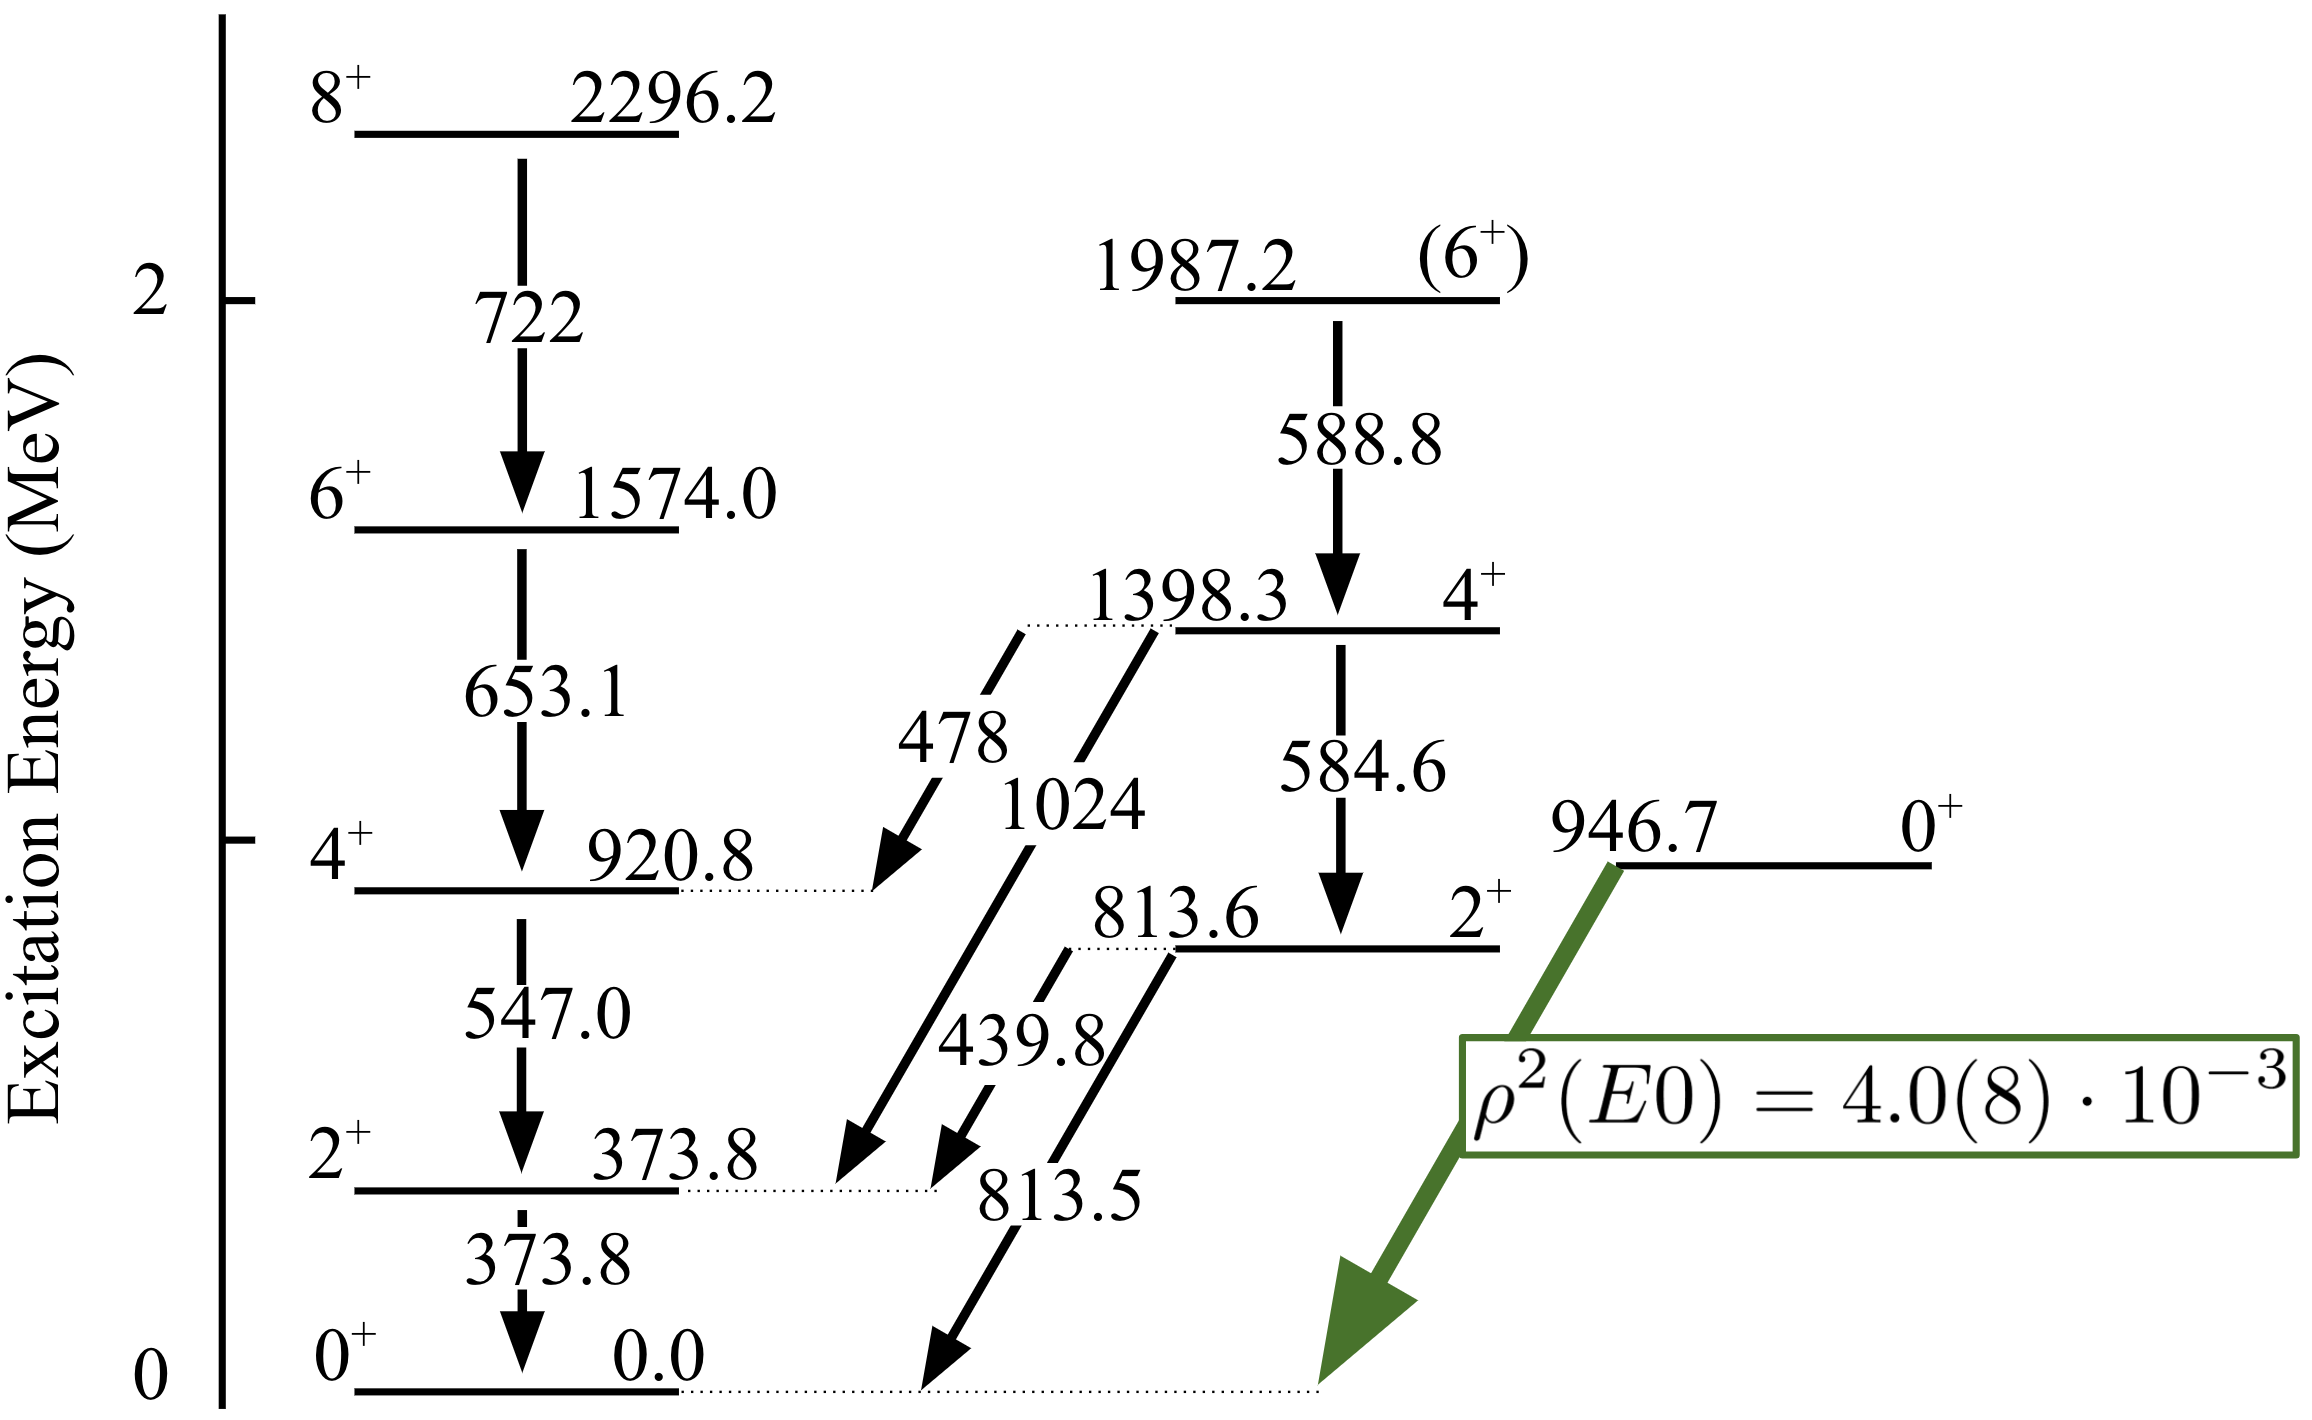
\includegraphics[width=\textwidth]{intro_110Pd_E0.png}
  \caption[Partial level scheme for the nucleus $^{110}$Pd with a previous measurement of $\rho^2(E0)$ highlighted.]{Energy levels from the first three intrinsic excitations for the nucleus $^{110}\mathrm{Pd}$ \cite{ENSDF110Pd}. State and transition energies are given in keV. The spin and parity of each state is labeled. A previous measurement of $\rho^2(E0)$ for the $0^+_2 \rightarrow 0^+_1$ transition is listed \cite{Kibedi2005}.}
  \label{figure: levels of 110Pd}
\end{figure}

This previous measurement reveals a relatively weak $E0$ transition strength for the $0_2^+ \rightarrow 0^+_1$ transition. This transition is between two intrinsic excitation bands in which the lowest energy state has a nuclear spin of 0. Different bands in a nucleus can be described by their angular momentum projection onto the axis of symmetry (the $K$ quantum number). An individual band's $K$ value is given by the nuclear spin assignment of its lowest energy level. Generally $E0$ transitions have a $\Delta K = 0$ selection rule, and the expectation was to see a low value for $\rho^2(E0)$ in the $2^+_2 \rightarrow 2^+_1$ transition \cite{CastenText}. 

In Chapter 2 the theory of the nuclear shell model, and nuclear state mixing is discussed. The modes of transition that exist for a decaying nucleus and their correspondence to nuclear properties is outlined. The experimental setup and the analysis techniques are detailed in Chapter 3. The results of the experiment are presented and discussed in Chapter 4. This work is brought to conclusion in Chapter 5, and the opportunity for potential future research is highlighted.

\endinput

Any text after an \endinput is ignored.
You could put scraps here or things in progress.

In such a transition, the dominant mode of decay is the emission of an orbital $e^-$ from the atom. This process is called internal conversion, and the electrons produced are called internal conversion electrons. Here the spatial overlap of nuclear wave functions with that of the orbital $e^-$ results in a transfer of energy to, and subsequent ejection of the $e^-$ from the atom. Given the shell structure of atomic electrons, this decay mode is most probable to occur by emission of the nearest, K shell electrons, with descending probability for shells at successively further distances from the nuclear core.

While internal conversion is the only decay mode available in these unique, zero-angular-momentum-vector-difference transitions, it is a competitive process to \gr emission in all other transitions. 


%%    2. Main body
%% Generally recommended to put each chapter into a separate file
%% \include{relatedwork}
%% \include{model}
%% \include{impl}
%% \include{discussion}
%% \include{conclusions}
%% The following is a directive for TeXShop to indicate the main file
%%!TEX root = diss.tex

%%%%%%%%%%%%%%%%%%%%%%%%%%%%%%%%%%%%%%%%
\chapter{Theory}
\label{ch:Theory}
%%%%%%%%%%%%%%%%%%%%%%%%%%%%%%%%%%%%%%%%

The observation of the radiation emitted during nuclear decay can lead to a determination of nuclear properties and structure. As nuclei decay, they emit radiation most probably in the form of $\gamma$-ray photons. Nuclei can also decay via the emission of an orbital electron ($e^-$). The quantitative analysis of these different types of decay allows for comparison to models of nuclear behaviour that attempt to predict such processes. The development of these models help explain nuclear decay, and the configurations that nuclei can inhabit. Transition strengths in particular can serve as stringent tests of nuclear models, delineating the parameter spaces in which they either are, or are not applicable. Generally, the forces within the nucleus compose a difficult modeling problem by virtue of the number of interacting particles that must be considered. Attempts to do so rely on approximations. The nuclear shell model provides an accurate description of many nuclei, and their behaviours, but falls short of describing how the nucleons act in unison. Further treatments, such as the liquid drop model, provide a closer interpretation of nuclear collectivity \cite{KraneText}.  

%%%%%%%%%%%%%%%%%%%%%%%%%%%%%%%%%%%%%%%%
\section{The Nuclear Shell Model}
%%%%%%%%%%%%%%%%%%%%%%%%%%%%%%%%%%%%%%%%

In the atomic model, orbiting electrons are subdivided into discrete shells wherein each shell is filled, beginning with the lowest energy level. This filling of shells must not violate the Pauli exclusion principle, which stipulates that two or more electrons cannot occupy the same quantum state simultaneously. Similar evidence exists for a shell structure in the nucleus, where neutrons and protons exist in independent, discrete shells.

A prime example of this evidence is the two-neutron separation energy, $S_{2n}$, as a function of nucleon number, shown in Figure \ref{figure: two neutron separation energy plot} \cite{KraneText,EvittsParse}. The two-neutron separation refers to the energy required to remove two neutrons from a nucleus. It is the nuclear analogue to single electron removal from an atomic shell, with two nucleons considered due to pairing effects between nucleons. The $S_{2n}$ values follow large steps downward following the closing of a nuclear shell, which occurs following nucleon numbers of 8, 20, 28, 50, 82 and 126. The nucleon numbers where these drops in $S_{2n}$ occur are collectively known as the magic numbers.

\begin{figure}[!ht]
  \centering
  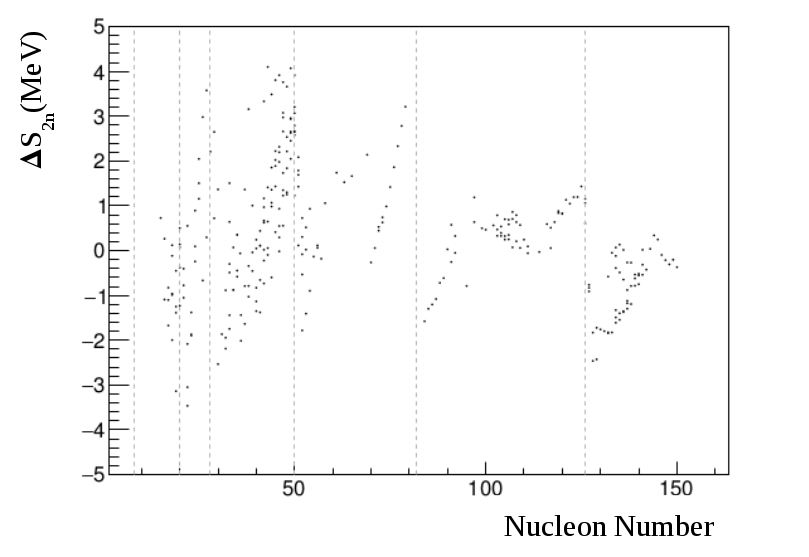
\includegraphics[width=\textwidth]{theory_two_neutron.png}
  \caption[The difference between the experimental two-neutron separation energy, $S_{2n}$, parsed from the evaluated nuclear data sheets \cite{EvittsParse} and the value obtained from the semi-empirical mass formula \cite{KraneText}.]{The difference between the experimental two-neutron separation energy, $S_{2n}$, parsed from the evaluated nuclear data sheets \cite{EvittsParse} and the value obtained from the semi-empirical mass formula \cite{KraneText}. The parameters used here are 15.5 MeV for the volume term, 16.8 MeV for the surface term, 0.72 MeV for the Coulomb term, 23 MeV for the symmetry term and 34 MeV for the pairing term \cite{KraneText}. The magic numbers of 8, 20, 28, 50, 82 and 126 are shown by the grey dashed lines where there are sudden drops. Image from \cite{EvittsThesis}.}
  \label{figure: two neutron separation energy plot}
\end{figure}

Characterization of the sequence of nuclear energy levels requires a treatment within the formalism of quantum mechanics. The nuclear potential is a combination of a strong force interaction between all nucleons, and a coulomb interaction between the positively charged protons \cite{CastenText}. The shear degree of inter-nucleon interaction terms that must be considered makes this an insoluble problem by explicit analytic means. As an approximation, the harmonic oscillator potential provides a reasonable starting point. The potential $V(r)$ is given by \cite{CastenText}

\begin{align}
	V(r) = \frac{1}{2}m\omega^2r^2
	\label{equation: harmonic oscillator potential}
\end{align}

where $m$ is the mass of the nucleon, $\omega$ is the oscillating frequency, and $r$ denotes the radius. Inserting this potential into the three-dimensional Schr\"odinger equation

\begin{equation}
\Bigg[\frac{-\hbar^2}{2m}\nabla^2+V(r)\Bigg]\Psi(r) = E\Psi(r)
\label{equation: 3D schrodinger}
\end{equation}

yields an analytic solution for the energy levels, as desired.  But this approximation fails to reproduce the characteristic magic numbers for nucleon shell closures, as observed experimentally. A more appropriate approximation can be made by modeling the nuclear potential as a mean field. This theoretical model replicates the approximate charge distribution of the nucleus, with the central region constant \cite{CastenText}. This potential, known as the Woods-Saxon potential, is of the form

\begin{equation}
V(r) = \frac{-V_0}{1+\mathrm{exp}[(r-R)/a]}
\label{equation: woods-saxon potential}
\end{equation}

where the strength of the potential is a function of r, the radial distance from the origin. $R = A^{1/3}\mskip\thinmuskip \mathrm{fm}$ is the mean radius of a nucleus, $A$ is the atomic mass number, $a=\SI{0.524}{fm}$ is the skin thickness (i.e. the radius of the nucleus in which the charge density decreases from $90\%$ of its value to $10\%$), and $V_0$ is an adjustable parameter in order to replicate the correct separation energies \cite{KraneText}. Additionally, a spin-orbit coupling force must be included in the potential. This force is an interaction between the intrinsic nuclear spin of the nucleon, and its orbital angular momentum. In short, increasing degree of alignment between the nucleon's spin and angular momentum will increase the attractiveness of the potential. Substituting this complete potential into the three-dimensional Schr\"odinger equation is capable of reproducing the magic numbers that we observe experimentally. The energy levels yielded by these subsequent approximation attempts are shown in Figure \ref{figure: energy level solutions for three potentials} \cite{KraneText}. An energy level is defined by the label ``$nl$" where $l$ is the orbital angular momentum denoted by a letter i.e. $s, \ p, \ d, \ f,$ corresponds to values 0, 1, 2, and 3 respectively. The number $n$ is an index denoting the $n^\mathrm{th}$ occurrence of a level with that particular $l$ value, starting from $n=0$. The parity of a state, $\pi$, is determined by $(-1)^l$. Each level can contain a maximum of 2(2$l$+1) nucleons, due to degeneracy of both $s$ and $m$, representing the spin and magnetic quantum numbers \cite{KraneText}.  

\begin{figure}[!ht]
  \centering
  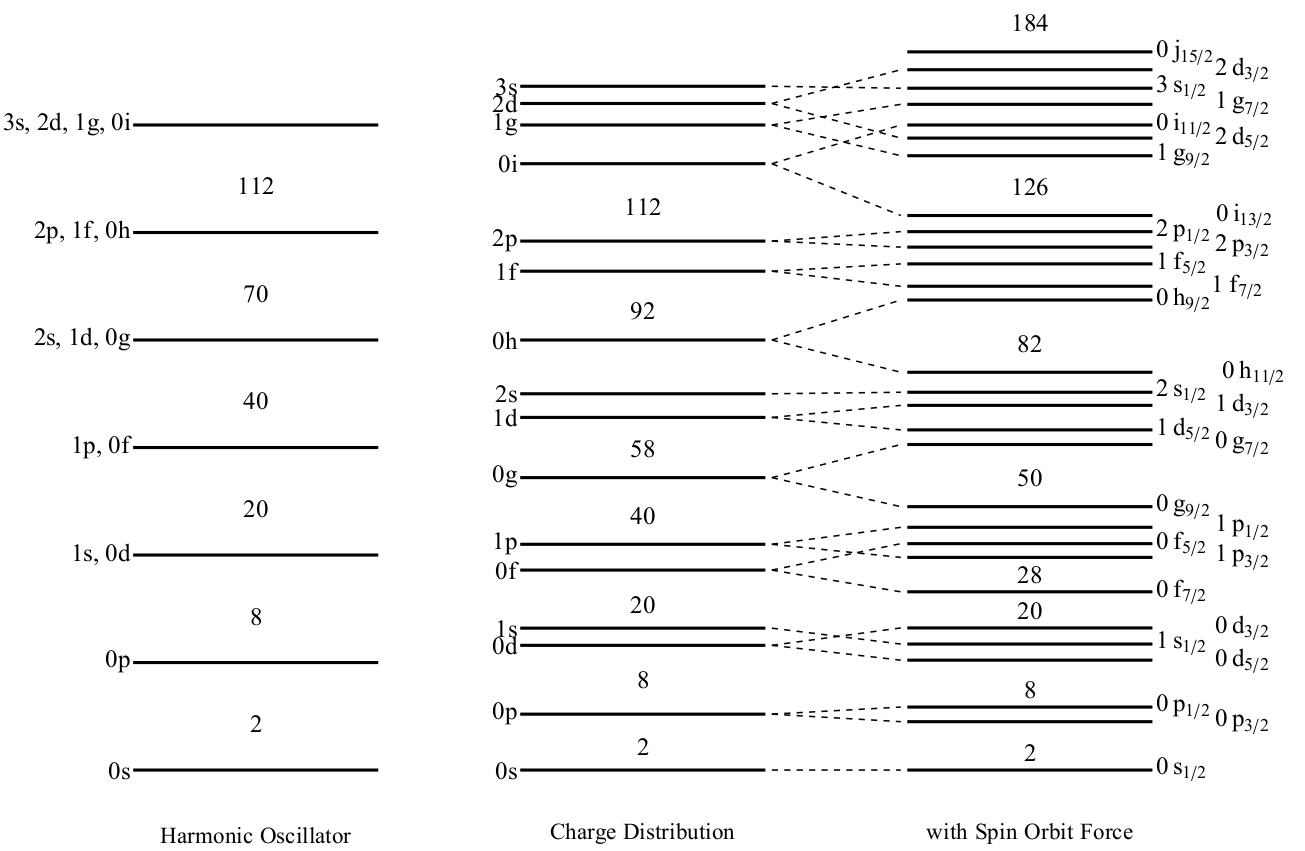
\includegraphics[width=\textwidth]{theory_schrodinger_energies.png}
  \caption[The energy levels yielded by solving the 3-D Schr\"odinger Equation (\ref{equation: 3D schrodinger}) for three different theoretical energy potential approximations: harmonic oscillator, Woods-Saxon, and Woods-Saxon with spin-orbit coupling.]{The energy levels yielded by solving the 3-D Schr\"odinger Equation (\ref{equation: 3D schrodinger}) for three different theoretical energy potential approximations: harmonic oscillator, Woods-Saxon, and Woods-Saxon with spin-orbit coupling. The number between particular levels is the number of nucleons required to fill a major shell. Only after the inclusion of the spin-orbit coupling interaction are the empirically observed magic numbers reproduced. Image from \cite{EvittsThesis}.}
  \label{figure: energy level solutions for three potentials}
\end{figure}

%%%%%%%%%%%%%%%%%%%%%%%%%%%%%%%%%%%%%%%%
\section{The Mixing of Nuclear States}
%%%%%%%%%%%%%%%%%%%%%%%%%%%%%%%%%%%%%%%%

Nuclei, being fundamentally quantum mechanical objects, exist in states that are best described as a linear combination of unperturbed states with equal spin and parity. Furthermore, there exists the potential for an interaction, $V$, between two mixed states. In Figure \ref{figure: diagram of two-state mixing model} two initial states are shown with energies $E_{1/2}$ and wavefunctions $\phi_{1/2}$. The interaction, $V$, between them results in a perturbation of their energies and wavefunctions. The resulting states are labelled by energies $E_{\mathrm{I/II}}$ and wavefunctions $\psi_{\mathrm{I/II}}$  \cite{KraneText}. 

\begin{figure}[!ht]
  \centering
  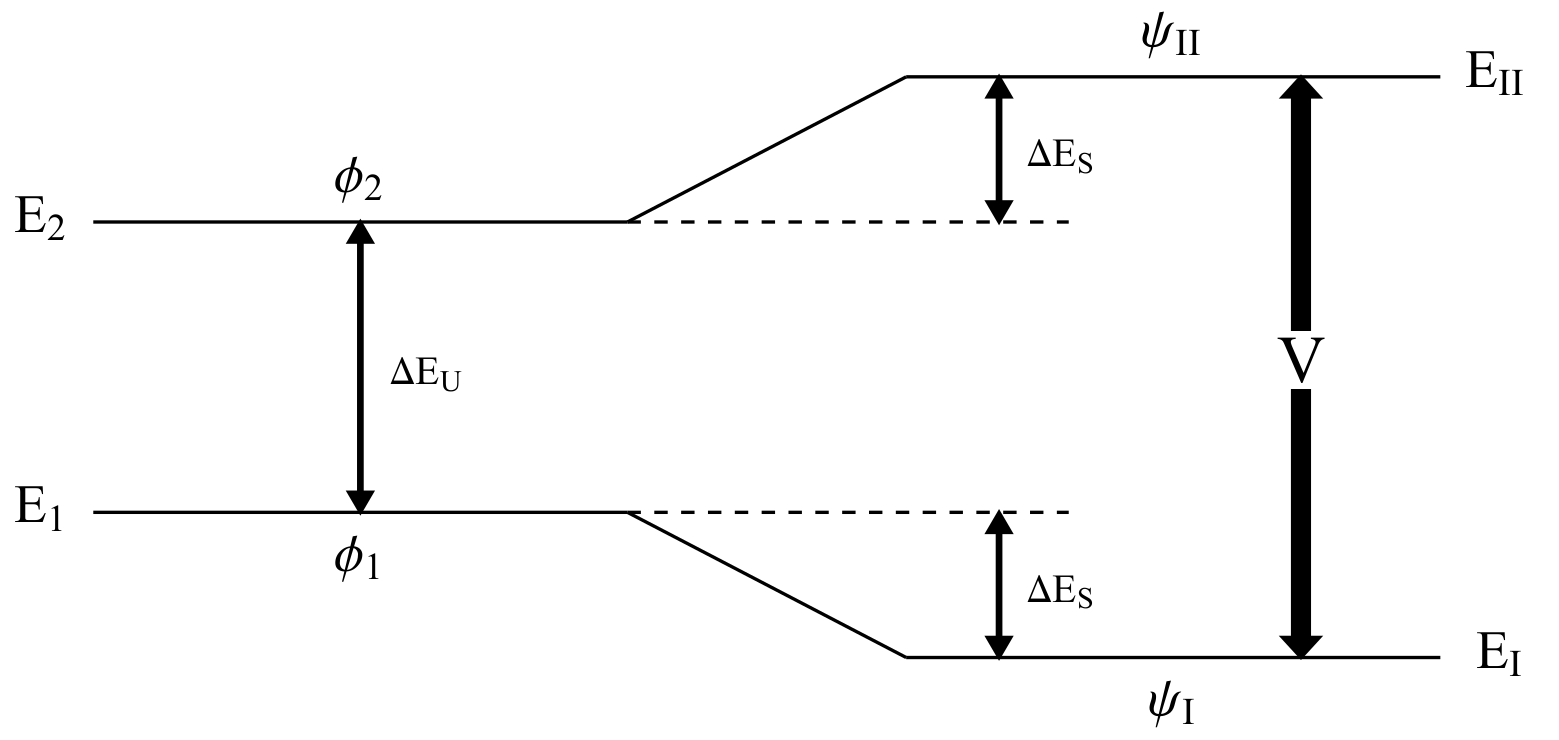
\includegraphics[width=\textwidth]{theory_mixing_diagram.png}
  \caption[Diagram of a two-state mixing interaction \cite{KraneText}. Image from \cite{EvittsThesis}.]{Diagram of a two-state mixing interaction \cite{KraneText}. Image from \cite{EvittsThesis}.}
  \label{figure: diagram of two-state mixing model}
\end{figure}

These new wavefunctions can be described by the degree of mixing that occurs between the original states. In the following expressions:

\begin{equation}
\begin{aligned}
\psi_\mathrm{I} = & a\phi_1 + b\phi_2 \\
\psi_\mathrm{II} = & -b\phi_1 + a\phi_2 \\
\label{equation: wavefunctions of mixed states}
\end{aligned}
\end{equation}

where $a$ and $b$ are the mixing amplitudes with normalization such that $a^2 + b^2 = 1$. If we consider the wavefunctions of the two unperturbed states, $\phi_{1/2}$, within energy space, then the closer the energies of these two states are, the greater degree of overlap will exist between the two wavefunctions. Hence, the strength of the mixing is a function of both the size of the interaction, $V$, and the size of the gap between the two energies, $E_{1/2}$. The ratio $R = \Delta E_\mathrm{U}/V$ encapsulates these two contributions, where $E_\mathrm{U}$ is the unperturbed energy difference as pictured in Figure \ref{figure: diagram of two-state mixing model} \cite{CastenText}. The energy difference following the interaction perturbation, $E_\mathrm{P}$, can be related to to $E_\mathrm{U}$ and $R$ by

\begin{equation}
\frac{\Delta E_\mathrm{P}}{\Delta E_\mathrm{U}} = \sqrt{1+\frac{4}{R^2}}
\label{equation: two state mixing energy gaps and strength}
\end{equation}

and the total shift in energy undergone by one of the states, $\Delta E_\mathrm{S}$, is given by

\begin{equation}
\frac{\lvert \Delta E_\mathrm{P} \rvert}{\Delta E_\mathrm{U}} = \frac{1}{2}\Bigg[\sqrt{1+\frac{4}{R^2}}-1\Bigg]
\label{equation: two state mixing - single state energy shift}
\end{equation}

A lower limit on the mixing amplitude $b$ can be expressed in terms of the ratio, $R$, as follows

\begin{equation}
b = \frac{1}{\sqrt{1+\Big[R/2+\sqrt{1+R^2/4}\Big]^2}}
\label{equation: two state mixing - amplitude b in terms of R}
\end{equation}

An interpretation of mixing as it relates to the two aforementioned physical contributions, unperturbed energy gap and interaction magnitude, can be gleaned from this expression. As the energy gap between the unperturbed states is increased relative to the interaction strength, the resulting $R$ value becomes large. Substituted into Equations (\ref{equation: two state mixing - single state energy shift}) and (\ref{equation: two state mixing - amplitude b in terms of R}) yields small values of $b$ and $\Delta E_\mathrm{S}$. With a negligible $\Delta E_\mathrm{S}$ value, Equation (\ref{equation: two state mixing - amplitude b in terms of R}) becomes purely a function of the interaction strength, $V$, i.e. it becomes possible to calculate $V$ from an experimental measurement of $b$. In the inverse situation, with large interaction and small unperturbed energy gap (i.e. $\Delta E_\mathrm{U} \approx 0$) then the states following the consideration of mixing become $E_\mathrm{I/II} = E_0 + V$, where each state is merely shifted from its initial energy, $E_0$, by the interaction strength only. This demonstrates that in any two-state mixing scenario, the observed energy difference between the two states may never be smaller than twice the interaction strength \cite{CastenText}. 

%%%%%%%%%%%%%%%%%%%%%%%%%%%%%%%%%%%%%%%%
\section{Collective Models of Nuclear Structure}
%%%%%%%%%%%%%%%%%%%%%%%%%%%%%%%%%%%%%%%%

While the nuclear shell model is an appropriate approximation for nuclei that have closed shells, it begins to lose applicability as the number of valence nucleons increases. For these regions an alternative model may be used that focuses on the collective nature of the nucleus. In non-spherical nuclei the deformation parameter, $\beta$ may be related to the eccentricity of the ellipsoid by

\begin{gather}
\beta = \frac{4}{3}\sqrt{\frac{\pi}{5}}\frac{\Delta R}{R_{\mathrm{AVG}}}
\label{equation: beta and spheroids}
\end{gather}

where $\Delta R$ is the difference between the semi-major and semi-minor axes of the ellipsoid and $R_\mathrm{AVG}=1.3A^{1/3} \si{fm}$, with $A$ being the atomic mass number. When $\beta>0$ the nucleus is prolate, and when $\beta<0$ the nucleus is oblate \cite{KraneText}. The excitation energies of an idealized deformed, axially-symmetric rotating nucleus are given be

\begin{gather}
E = \frac{\hbar^2}{2I}J(J+1)
\label{equation: rotational energies as function of J}
\end{gather}

where $I$ is the moment of inertia. The addition of rotational energy results in higher excited states with larger spin. Equation (\ref{equation: rotational energies as function of J}) is used to determine the idealized excitation energies of higher lying states; for example, in a nucleus of even number of protons and even number of neutrons the ground state is $0^+$ and the energies are

\begin{equation}
\begin{aligned}
E(0^+) ={} & 0 \\
E(2^+) ={} & 6(\hbar/2I) \\
E(4^+) ={} & 20(\hbar/2I)
\label{equation: three rotational energies calculated}
\end{aligned}
\end{equation}

Thus, the ratio of $4^+_1/2^+_1$ energies in a rigidly-deformed rotational nucleus is 3.33. Only even values of $J$ are considered due to the coupling of an even number of spins within the nucleus \cite{KraneText}. Generally, the ratio of $4^+_1/2^+_1$ energies is an indication of the macroscopic behaviour of the nucleus. In the regions between closed shells, this ratio ranges from 3.33 in rotational nuclei to 2.0 for nuclei that behave as spherical vibrators. Nuclei with intermediate values are described as the transitional nuclei between these two idealized cases. A chart of the nuclides is shown in Figure \ref{figure: 4 to 2 ratio across the chart} which displays the ratio of $4^+_1$ to $2^+_1$ energies. The magic numbers are highlighted as grey dashed lines. Red points correspond to a spherical vibrator where the ratio is close to 2.0 and the blue points are rotational nuclei where the ratio approaches 3.33. In the intermediate yellow region, a gradient of different configurations exists which are referred to as transitional nuclides. It can generally be concluded from Figure \ref{figure: 4 to 2 ratio across the chart} that the rotational nuclei exist in the regions between closed shells whereas the spherical vibrator nuclei are low mass (commensurate with low total nucleon number) or close to the magic numbers \cite{EvittsParse}. 

\begin{figure}[!ht]
  \centering
  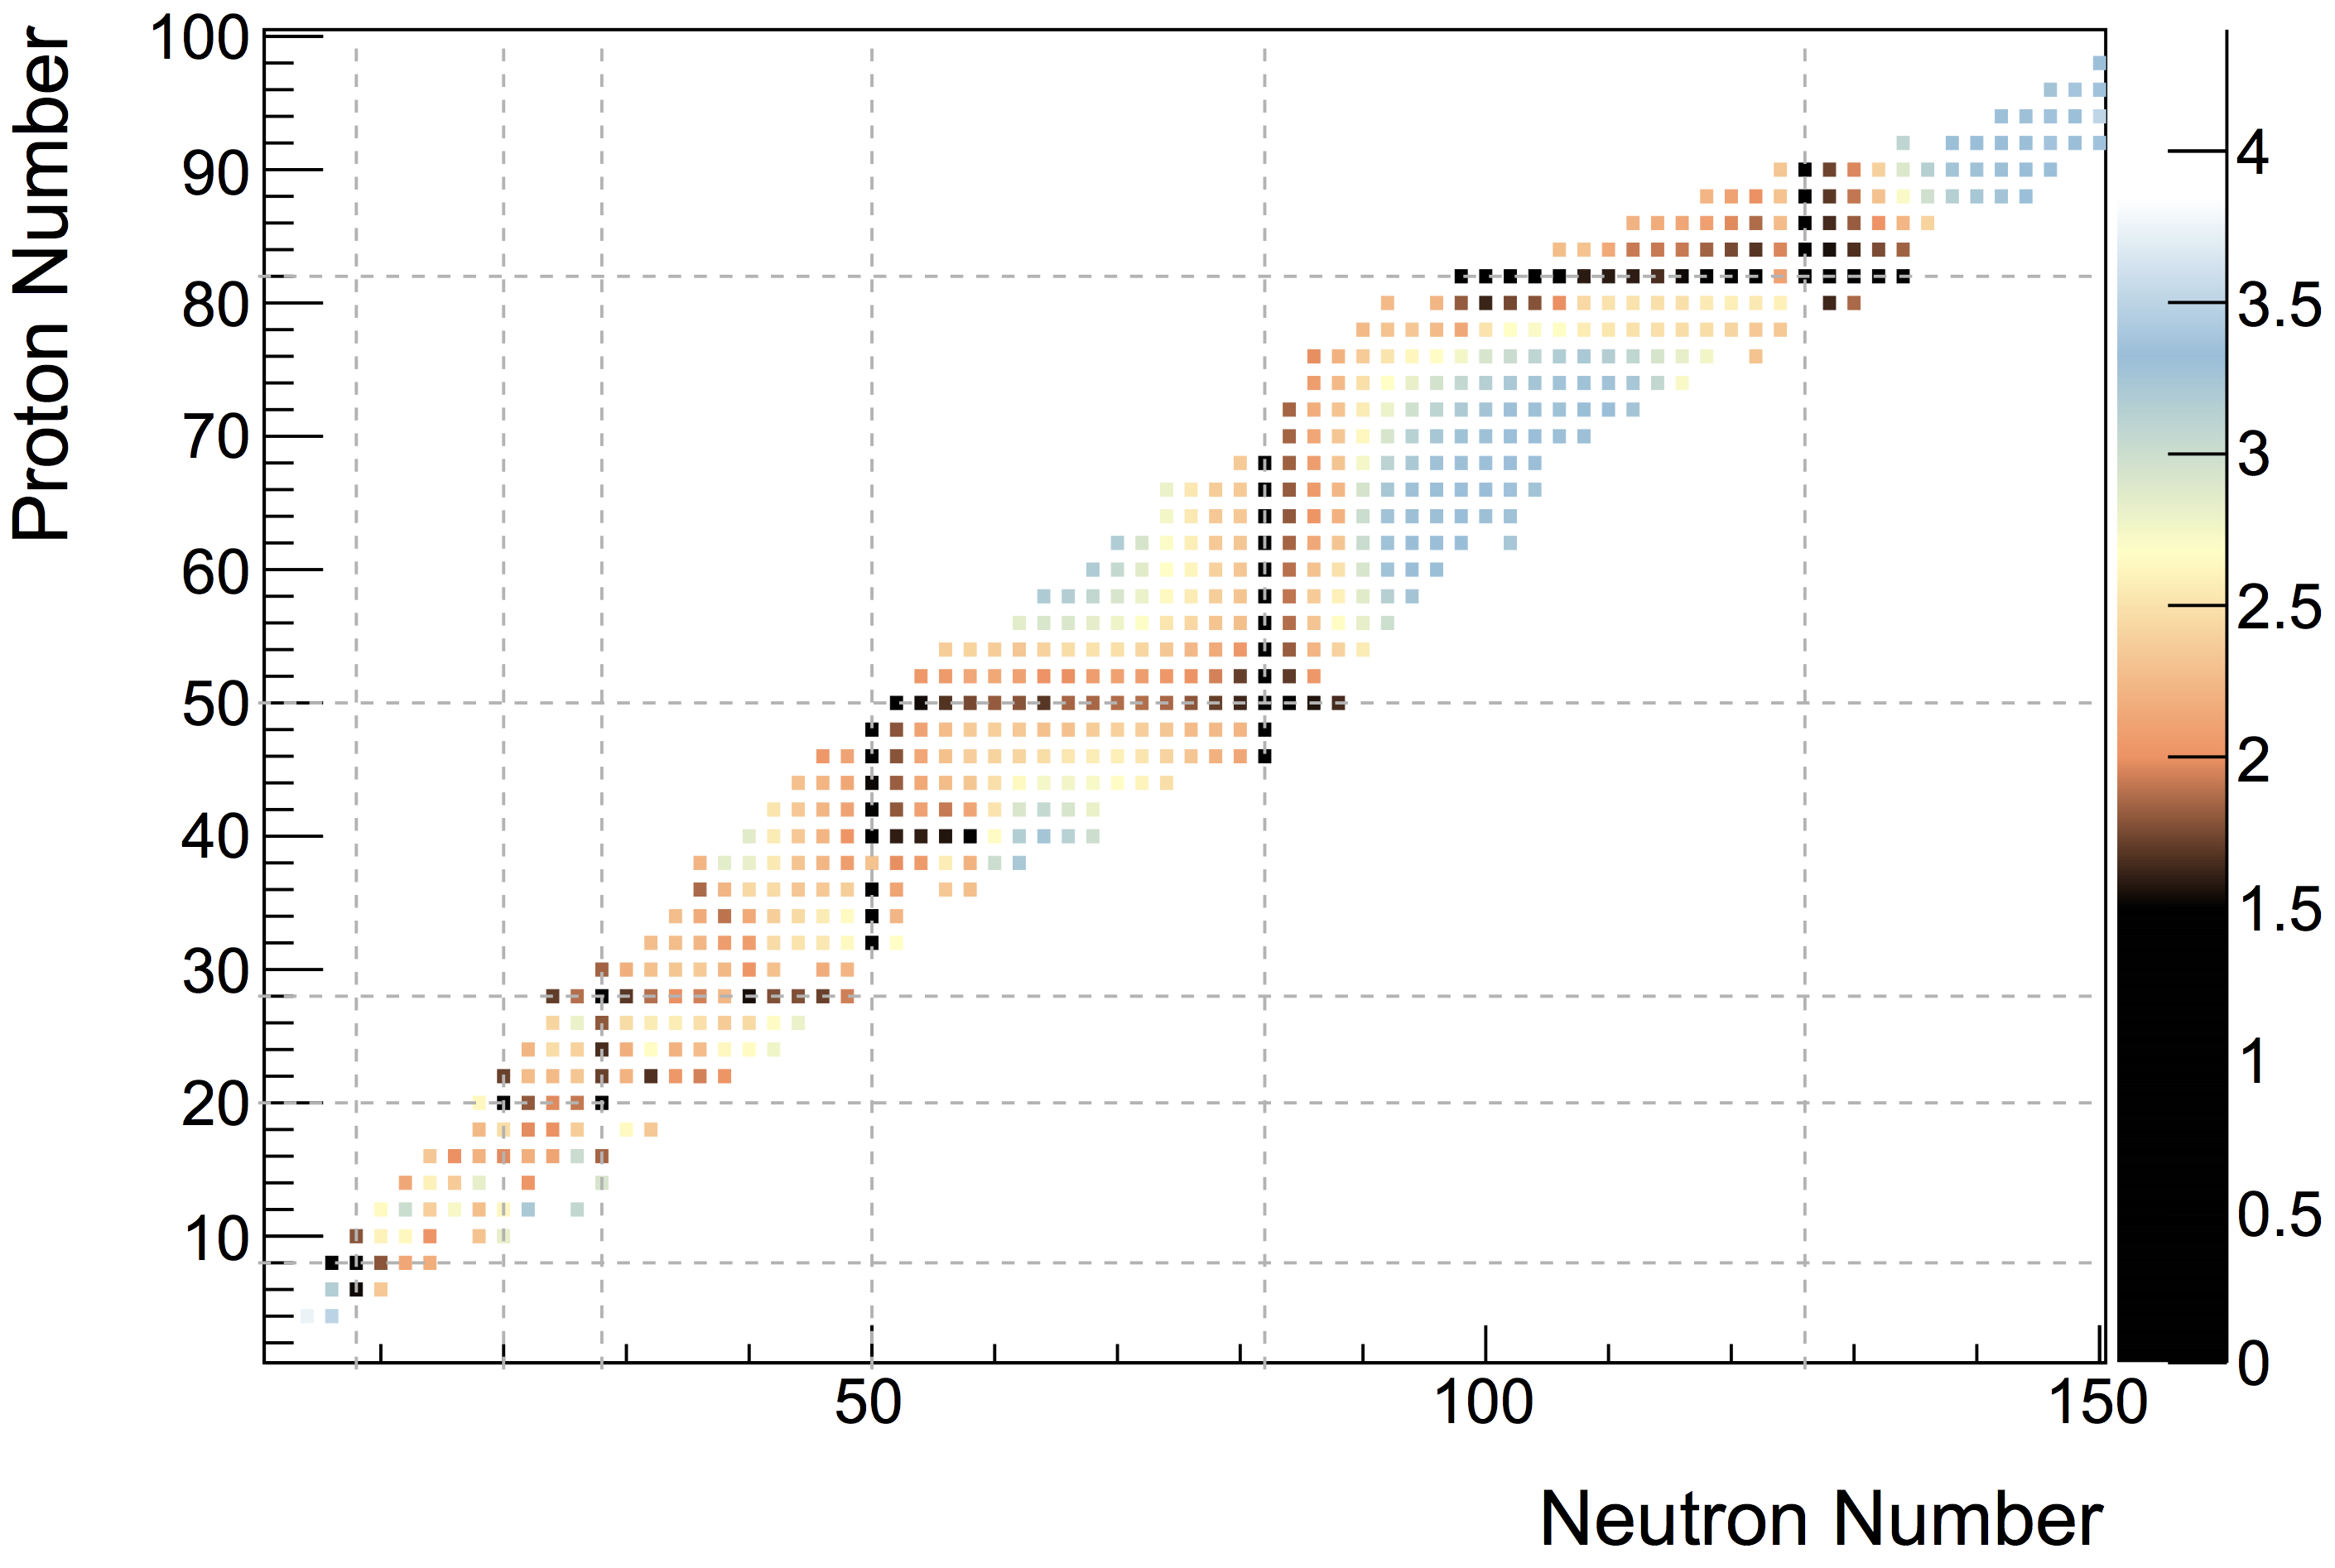
\includegraphics[width=\textwidth]{theory_4to2_chart.png}
  \caption[The ratio of $4^+_1$ to $2^+_1$ empirical energies for each nuclide across the chart \cite{EvittsParse}.]{The ratio of $4^+_1$ to $2^+_1$ empirical energies for each nuclide across the chart \cite{EvittsParse}. The magic numbers are shown by grey dashed lines. The red points correspond to a spherical vibrator, the blue are rotational, and the yellow are the transitional nuclei between the two. Image from \cite{EvittsThesis}.}
  \label{figure: 4 to 2 ratio across the chart}
\end{figure}

%%%%%%%%%%%%%%%%%%%%%%%%%%%%%%%%%%%%%%%%
\subsection{Shape Coexistence}
%%%%%%%%%%%%%%%%%%%%%%%%%%%%%%%%%%%%%%%%

The phenomenon of shape coexistence refers to a quantum mechanical behaviour, where a single nucleus simultaneously inhabits two or more possible configurations. Recalling the two-state mixing model, when two nuclear states of the same spin and parity (with similar excitation energies) but two different intrinsic shapes exist as an admixture, we can describe the situation as one of shape coexistence. 

If all possible configurations of nucleons within the nuclear volume are considered, and for each such configuration the inter-nuclear energy potential is plotted, then an energy potential surface is developed. In Figure \ref{figure: famous Pb figure} such a potential energy surface is plotted for the spin-zero states of the nucleus $^{186}\mathrm{Pb}$ \cite{Duguet2003}. The degree of spheroid deformation, expressed in terms of the parameter $\beta$ discussed earlier, varies along the $x$ and $y$ axes. The corresponding energy potential within the nucleus is plotted as the height, $z$. Hence, we see three distinct minima in the potential surface, each representing a potential nuclear shape that is part of the coexisting admixture. 

\begin{figure}[!ht]
  \centering
  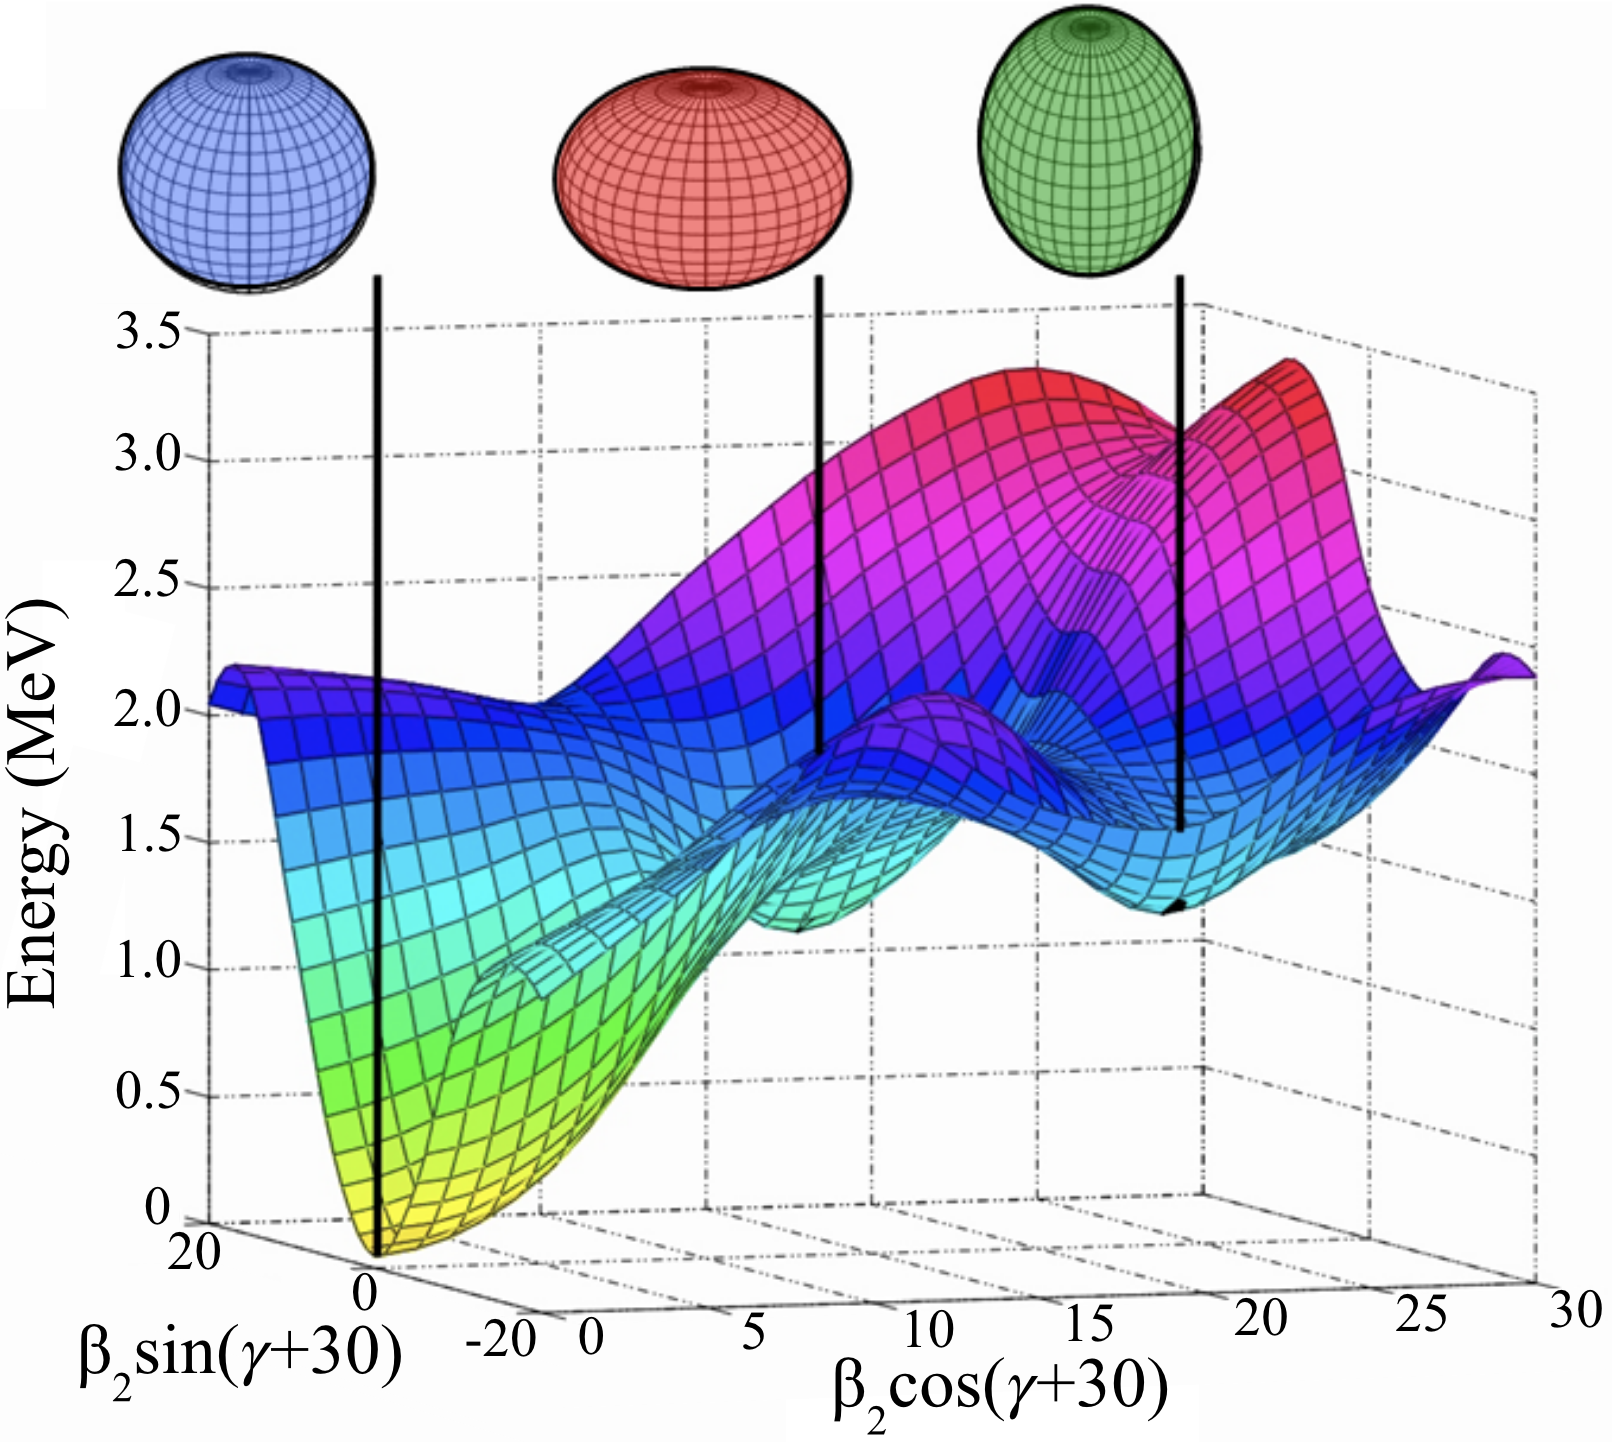
\includegraphics[width=0.7\textwidth]{theory_Pb_shape.png}
  \caption[The potential energy surface for $^{186}\mathrm{Pb}$ is plotted as a function of nuclear shape deformation. Three distinct minima, corresponding to three distinct nuclear structures, are highlighted.]{The potential energy surface for $^{186}\mathrm{Pb}$ is plotted as a function of nuclear shape deformation. The $x$ and $y$ axes correspond to deformations along the spheroid axes, in turn corresponding to reconfigurations of the constituent nucleons. The $\gamma$ parameter relates to the degree of triaxiality in the deformation (that is, the relative lengths of the three principal axes of the spheroidal nucleus). Three differently shaped spin-zero states are denoted by three distinct minima in the potential energy surface \cite{Duguet2003}.}
  \label{figure: famous Pb figure}
\end{figure}

%%%%%%%%%%%%%%%%%%%%%%%%%%%%%%%%%%%%%%%%
\section{Nuclear Reactions}
%%%%%%%%%%%%%%%%%%%%%%%%%%%%%%%%%%%%%%%%

Following a nuclear interaction, a nucleus can be left in a number of excited energy states. The reaction typically achieves a transfer of energy to the nucleus as part of a collision. These collisions can be categorized based on the degree of inter-penetration of the interacting nuclear volumes, which then corresponds to the force mechanism by which the interaction is mediated. In a collision where the colliding nuclei interact only electromagnetically, that is their position wavefunctions do not breach the short range within which the strong force applies, then the interaction mechanism is purely that of coulomb excitation. The nuclei themselves cannot be constitutively changed by this type of collision. In a pure Coulomb interaction, the interacting nuclei have only the possibility of being excited into low-lying energy states by the electromagnetic field. 

A nuclear collision that occurs at high enough energy such that strong force interactions occur, where the pure-coulomb interaction range is exceeded, is described as a ``beyond-barrier" collision. The interaction of the strong force from the different nucleons can lead to constitutive changes in nuclear structure, and not only are nuclei excited to higher lying states, but they also can exchange particles. 

From an experimental perspective, there are trade-offs between the different methods of populating the excited states of nuclei, dependent upon the desired observables for measurement. 

%%%%%%%%%%%%%%%%%%%%%%%%%%%%%%%%%%%%%%%%
\section{Gamma Decay}
%%%%%%%%%%%%%%%%%%%%%%%%%%%%%%%%%%%%%%%%

When excited nuclear states decay, they do so through transitions involving energy emission. The energy emitted from the nucleus may be in the form of photons, or particles. The dominant way that this occurs is through the emission of $\gamma$ rays. An emitted $\gamma$ ray will carry away energy equal to the difference in energy between the initial and final states of the transition. The emitted gamma rays can be characterized by the electromagnetic multipolarity of the associated transition. These multipolarities define the angular momentum, parity and angular distribution of the gamma ray emission in space. The angular momentum of the nuclear transition, and subsequently the $\gamma$ ray emitted, is governed by a set of selection rules, in conjunction with the parity \cite{KraneText}.

If the spin and parity of the two nuclear energy levels is given by $J^{\pi_i}_{i}$ and $J^{\pi_f}_{f}$, then the angular momentum carried away by the $\gamma$ ray, $L$, can take values in the following range

\begin{equation}
|J_i-J_f|\leq L \leq J_i+J_f
\label{equation: gamma ray decay vector difference}
\end{equation}

Additionally, $\gamma$ rays must carry away at least 1 $\hbar$ unit of angular momentum, thus forbidding gamma ray emission as a mechanism for transitions between two nuclear states of spin-0. Transitions of this nature must occur by other mechanisms, such as internal conversion electrons or internal pair formation \cite{KraneText}. 
Electromagnetic multipole fields are classified as either electric or magnetic in nature according to specific parity rules. If an electric transition has even $L$ then there is no change in parity but if $L$ is odd then there is a change in parity. The inverse rule defines magnetic transitions. i.e.

\begin{equation}
\begin{aligned}
&\pi(EL)=(-1)^{L} \\
&\pi(ML)=(-1)^{L+1}
\label{equation: gamma ray decay selection rules}
\end{aligned}
\end{equation}

Combined, these selection rules define the allowed multipolarities for a given transition. For example, in a $2^+$ to $2^+$ transition, the $M1$, $E2$, $M3$ and $E4$ processes will all have non-zero probability. There is also the $E0$ transition available but this will not decay through the emission of a $\gamma$ ray and will instead decay through alternate methods such as internal conversion \cite{KraneText}. 

%%%%%%%%%%%%%%%%%%%%%%%%%%%%%%%%%%%%%%%%
\section{Internal Conversion Decay}
%%%%%%%%%%%%%%%%%%%%%%%%%%%%%%%%%%%%%%%%

$E0$ transitions cannot occur by $\gamma$ ray emission due to the requirement for the photon to carry at least one unit of angular momentum. These transitions must occur by alternate modes, such as the emission of two photons ($\gamma \gamma$), production of an electron-positron pair (internal pair formation, $\pi$), or internal conversion electron decay.
In internal conversion electron decay, energy is released via the emission of one of the orbital electrons, with energy equal to the transition energy less the binding energy of the particular atomic orbital, $B_e$, i.e.

\begin{gather}
T_e = T_\gamma - B_e
\label{equation: icc conservation of energy}
\end{gather}

The total decay probability of a nuclear transition is equal to the sum of probabilities for the individual decay modes i.e.

\begin{gather}
\lambda_t = \lambda_\gamma + \lambda_e + \lambda_{\gamma \gamma} + \lambda_\pi +...
\label{equation: total decay as constituent sum}
\end{gather}

This can be rearranged as

\begin{gather}
\lambda_t = \lambda_\gamma(1+\alpha_e+\alpha_{\gamma \gamma}+ \alpha_\pi+...)
\label{equation: re-arrange to define alpha icc}
\end{gather}

where $\alpha_x=\lambda_x/\lambda_\gamma$ is the coefficient of the specific decay mode, defined as a probability of that mode relative to $\gamma$ ray decay. $\alpha_e$ is the internal conversion coefficient \cite{KraneText}.

%%%%%%%%%%%%%%%%%%%%%%%%%%%%%%%%%%%%%%%%
\section{$E0$ Transitions}
%%%%%%%%%%%%%%%%%%%%%%%%%%%%%%%%%%%%%%%%

Examination of the individual strength of an $E0$ transition requires that the different transition multipolarities be deconvolved. The two dominant transition multipolarities present in a $2^+ \rightarrow 2^+$ transition are $M1$ and $E2$. The mixing ratio, $\delta(E2/M1)$, is defined such that the intensities of these multipolarities can be obtained from 

\begin{gather}
\lambda(E2) = \frac{\delta^2}{1+\delta^2} \\
\lambda(M1) = \frac{1}{1+\delta^2}
\label{equation: disambiguating the mixing ratio}
\end{gather} 

The $(E2/M1)$ mixing ratio and the internal conversion coefficient are both required for the calculation of $q^2$, which is the ratio of intensities between $E0$ and $E2$ transitions from a common initial state. It is given by $q^2 = I(E0)/I(E2)$. For a $2^+\rightarrow2^+$ transition, the mixing of $E0$, $M1$ and $E2$ components (higher $L$ components may be neglected) results in a $q^2$ determined by

\begin{gather}
q^2 = \frac{\alpha_\mathrm{exp}(1+\delta^2)-\alpha(M1)}{\alpha(E2)\cdot \delta^2}-1
\label{equation: squared}
\end{gather}

where $\alpha$ are theoretical conversion coefficients obtained from BrIcc \cite{KIBEDI2008202}, and $\alpha_\mathrm{exp}$ is an experimentally determined value of the internal conversion coefficient (i.e. ratio of $E0+M1+E2$ electrons vs. $M1+E2$ $\gamma$ rays). Using all of the available experimental inputs such as $q^2$, $\delta$, branching ratios and parent half-lives, then $\rho^2(E0)$ may be calculated from

\begin{gather}
\rho^2(E0) = \frac{1}{\Omega(E0) \cdot \tau(E0)}
\label{equation: E0 strength}
\end{gather}

where $\Omega$ is an electronic factor and $\tau(E0)$ is the partial mean lifetime of the $E0$ transition \cite{KIBEDI2008202}. 

The $E0$ transition strength can also be expressed in terms of the degree of mixing between different, coexisting shape states of the nucleus. Its sensitivity to shape coexistence in nuclei is best represented in  the following expression \cite{Wood1999}

\begin{gather}
\rho^2(E0) = \frac{Z^2}{R_0^4}a^2(1-a^2)\Big[\Delta \langle r^2 \rangle \Big]^2
\label{equation: E0 as probe of shape coexistence}
\end{gather}

where $Z$ is the proton number of the nucleus, $R_0$ is the nuclear radius of its hypothetical spherical configuration, $a$ is the degree of mixing between two possible states, and $\Delta \langle r^2 \rangle$ is the difference in the root-mean-squared charge radius of the two coexisting configurations. This gives the relevance of $\rho^2(E0)$ measurements explicitly within the terms of the nuclear structure context as developed thus far. 

\endinput

Any text after an \endinput is ignored.
You could put scraps here or things in progress.

% \begin{gather}
% \rho^2(E0) = q^2 \times \frac{\alpha_K(E2)}{\Omega_K(E0)} \times \frac{BR(E2_\gamma)}{\tau}
% \end{gather}
% where $\Omega_K(E0)$ is an electronic factor from atomic theory, $\tau$ is the lifetime of the parent state, and $BR(E2_\gamma)$ is the branching ratio of the $E2$ $\gamma$ ray transition. These latter two components are known values available on NNDC [!!! cite].

% \begin{gather}
% \tau(E0) = \frac{\Sigma \lambda_r}{\lambda_r(E0)}\cdot\tau
% \label{partialLifetime}
% \end{gather}
% where $\lambda_r$ is a relative decay constant and $\tau=T_{1/2}/\mathrm{ln}(2)$; $T_{1/2}$ is the half-life. \cite{KraneText}. This calculation requires a summation over every available decay mode from the parent state. 

\begin{equation}
\begin{aligned}
A_\eta(J_i L_1 L_2 J_f) ={} & \frac{1}{1+\delta^2}[f_\eta(J_f L_1 L_1 J_i)+ \\
					     & 2\delta f_\eta (J_f L_1 L_2 J_i)+     \\
                         & \delta^2 f_\eta (J_f L_2 L_2 J_i)]
\end{aligned}
\label{equation: angular distribution coefficient}
\end{equation}




110%% The following is a directive for TeXShop to indicate the main file
%%!TEX root = diss.tex

%%%%%%%%%%%%%%%%%%%%%%%%%%%%%%%%%%%%%%%%%%%%%%%%
\chapter{Experimental and Analysis Techniques}
\label{ch:techniques}
%%%%%%%%%%%%%%%%%%%%%%%%%%%%%%%%%%%%%%%%%%%%%%%%

The measurement of internal conversion coefficients depends on accurate analysis of $\gamma$-ray and electron spectra. For an individual transition between nuclear states, the relative transition probability by different transition modes must be calculated. This depends fundamentally on fitting mathematical functions to the spectroscopic peak structures that we have identified as belonging to specific transitions. This peak fitting is described in detail in Section \ref{sec: Peak Fitting}. The approach to calibrating the efficiencies of the detectors used in collection of the experimental data is then discussed in Section \ref{sec: Calibration of Detection Efficiency}. Calculations of previously unmeasured internal conversion coefficients must be normalized based on existing measurements, as well as the relative efficiency of our detectors. A simulated efficiency curve for the SPICE detector, using the GEANT4 toolkit, is discussed in Section \ref{sec: Simulated SPICE Efficiency}. This normalization, and the techniques used for determining internal conversion coefficients, are discussed in Section \ref{sec: Determining Internal Conversion Coefficients}. The calculation of electric monopole transition strengths, $\rho^2(E0)$, and associated error analysis are discussed in Section \ref{sec:Determining E0 Transition Strengths}.

%%%%%%%%%%%%%%%%%%%%%%%%%%%%%%%%%%%%%%%%%%%%%%%%
\section{Experimental Details}
\label{sec: Experimental Details}
% !!! For now this is mostly a copy of James' writing. This isn't the focus, so we're leaving it as is. It could easily be expanded using Daniel's style later.
%%%%%%%%%%%%%%%%%%%%%%%%%%%%%%%%%%%%%%%%%%%%%%%%

In June of 2016, a beam of 35.6\,MeV alpha particles with a typical intensity of 120\,ppA was delivered by the TRIUMF-ISAC-II superconducting linear accelerator to the TIGRESS spectrometer. The beam was incident on a self-supporting $^{110}$Pd target of 1.6\,mg/cm$^2$ with a 97.61\% isotopic enrichment. The target was positioned 8\,mm upstream of the nominal center of the TIGRESS spectrometer.

Two micron S3 silicon detectors of 140\,$\mu$m and 1000\,$\mu$m thickness were located downstream in a $\Delta E-E$ telescope configuration to detect and identify charged particles. Twelve of the TIGRESS high-purity germanium (HPGe) clover detectors were positioned around the target location to detect $\gamma$ rays. Four clovers were located at 45$^{\circ}$ with respect to the beam axis, and the remaining eight at 90$^{\circ}$ \cite{Hackman14}.

The spectrometer for internal conversion electrons (SPICE) detector was used to detect internal conversion electrons emitted from excited states populated in the reaction. The main detector of SPICE is a 6.1\,mm thick lithium-drifted silicon (Si(Li)) detector shielded by a photon shield from direct sight of the target. A magnetic lens formed of rare-earth permanent magnets collects and directs internal conversion electrons around the photon shield into the Si(Li) detector. The annular detector with inner and outer radii of 1 and 10\,cm is segmented into 120 individual segments arranged with 12 azimuthal sectors and 10 rings.

Figure \ref{figure: TIGRESS and SPICE schematic} provides a schematic diagram of the experimental setup, showing the incident $\alpha$ beam, TIGRESS, SPICE, the $^{110}$Pd target, and the downstream S3 detector.

\begin{figure}[!ht]
  \centering
  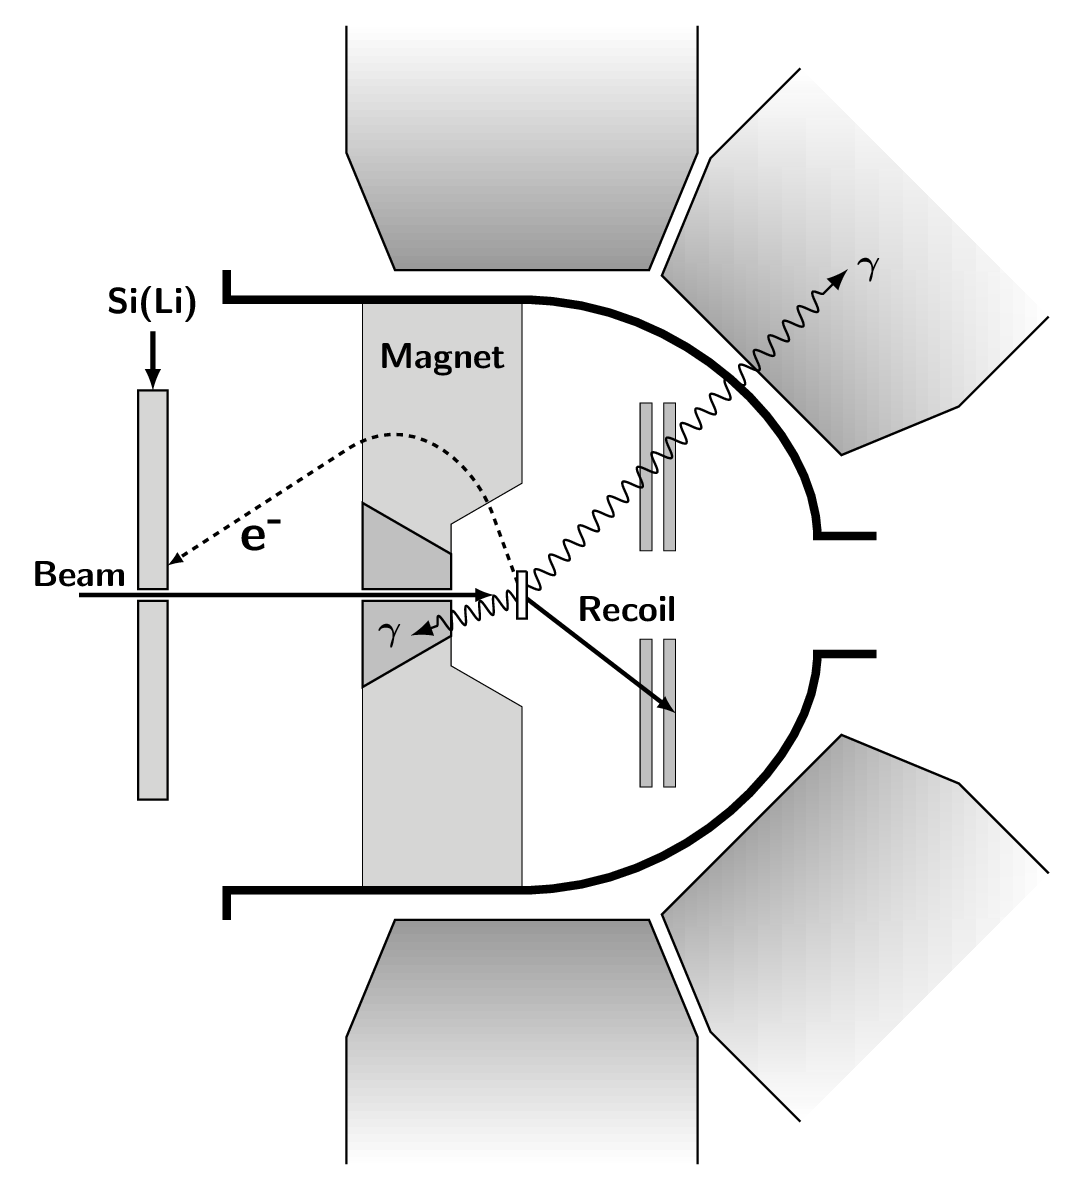
\includegraphics[width=0.8\textwidth]{techniques_spice_schematic.png}
  \caption[Schematic diagram of the experimental apparatus used in the June 2016 $\alpha$ particle scattering experiment at TRIUMF's ISAC-II facility.]{Schematic diagram of TIGRESS and SPICE in ISAC-II. An incoming beam of particles, $\alpha$ in this experiment, is shown colliding with the target, $^{110}\mathrm{Pd}$, at the center of the apparatus. As the excited target nuclei decay down to the ground state, they emit electrons ($e^-$) that follow curved trajectories through the internal magnetic fields of SPICE and are then detected by the upstream Si(Li) detectors. When $\gamma$-ray photons are emitted they are detected by the TIGRESS clovers, trapezoidal in the schematic, while the recoiling nuclei are detected by a downstream S3 silicon detector.}
  \label{figure: TIGRESS and SPICE schematic}
\end{figure}

Due to the above-Coulomb-barrier reaction energy of the collisions, excited nuclear states of several different nuclei were populated. Figure \ref{figure: nuclear chart region} shows the region of the nuclear chart where $^{110}\mathrm{Pd}$ and the other populated nuclei are found. The nuclei populated in this experiment are highlighted in orange.

\begin{figure}[!ht]
  \centering
  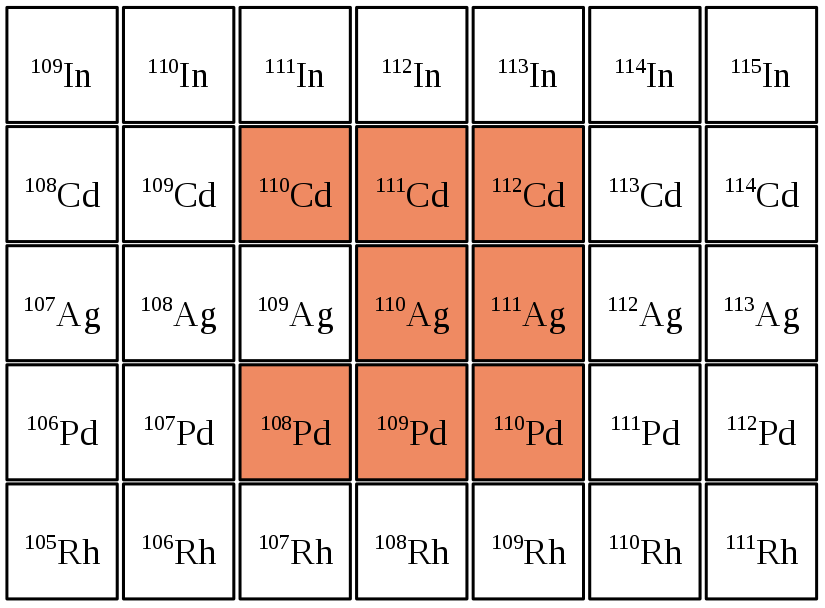
\includegraphics[width=0.7\textwidth]{techniques_chart_region.png}
  \caption[A chart of nuclides in the region of $^{110}\mathrm{Pd}$; highlighting the nuclei observed in the experiment.]{A chart of nuclides in the region of $^{110}\mathrm{Pd}$. The nuclei observed in this experiment are highlighted in orange.}
  \label{figure: nuclear chart region}
\end{figure}

The $\gamma$-ray and $e^-$ spectra for $^{110}$Pd is shown in Figure \ref{figure:spectrum_sample}. For both plots the spectrum presented is of all particles detected in time coincidence with a specific range of $\alpha$ particle energy, as detected in the S3. Three transitions are highlighted in each spectrum. All the denoted $e^-$ peaks are from $K$ shell electrons, except for the discernible $L$ shell peak from the $2^+_1 \rightarrow 0^+_1$ transition. 

\begin{figure}[!ht]
  \centering
  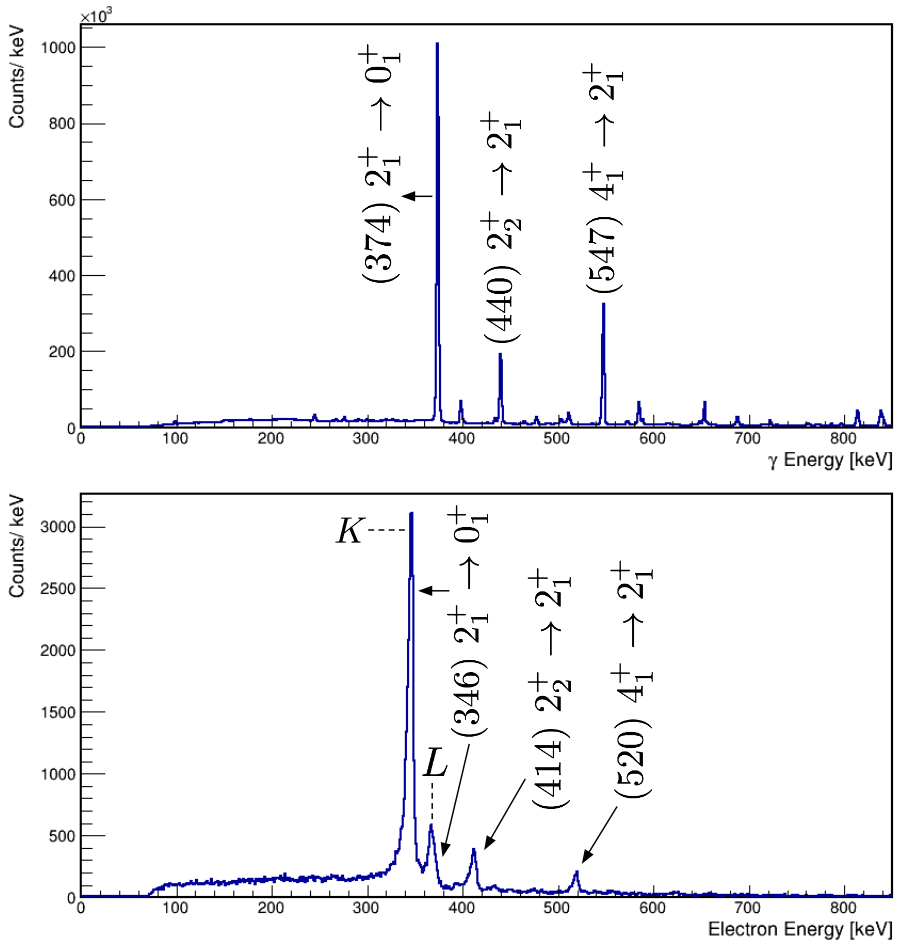
\includegraphics[width=0.9\textwidth]{techniques_alpha_spectra.png}
  \caption[The $\alpha$-particle gated $\gamma$-ray spectrum and the $\alpha$-particle gated $e^-$ spectrum.]{$\gamma$-ray and $e^-$ energy spectra for $^{110}$Pd from TIGRESS and SPICE. These spectra were produced by gating on a specific range of $\alpha$ particle energies, as detected in the S3 detector. Three transitions are highlighted in each spectrum, with the discernible $K$ and $L$ peaks for the $2^+_1 \rightarrow 0^+_1$ transition annotated. The energy listed for that transition, 346 keV, refers specifically to the $K$ peak.}
  \label{figure:spectrum_sample}
\end{figure}

%%%%%%%%%%%%%%%%%%%%%%%%%%%%%%%%%%%%%%%%%%%%%%%%
\section{Peak Fitting}
\label{sec: Peak Fitting}
%%%%%%%%%%%%%%%%%%%%%%%%%%%%%%%%%%%%%%%%%%%%%%%%

In both the $e^-$ and $\gamma$-ray spectra, the peaks have low-energy tails. This is due to incomplete charge collection in the detectors. The low energy tails of the $e^-$ peaks are likely to be due to target straggling and back-scattering. In both the $e^-$ and $\gamma$-ray spectra, the peak shapes may be described by regular Gaussian functions, $g(x)$, where

\begin{gather}
g(x) = e^{-\big(\frac{x-x_0}{\sigma \sqrt{2}}\big)^2}
\label{equation: Gaussian definition}
\end{gather}

summed with a skewed Gaussian, $d(x)$, to account for the low-energy tail from incomplete charge collection effects where

\begin{gather}
d(x) = e^{\big(\frac{x-x_0}{\beta}\big)} \cdot \mathrm{erfc}\Bigg[\frac{x-x_0}{\sigma \sqrt{2}} + \frac{\sigma}{\beta \sqrt{2}}\Bigg]
\label{equation: skewed Gaussian definition}
\end{gather}

where $x_0$ is the peak's centroid value, $\sigma$ is the width of the Gaussian and $\beta$ controls the length of the tail \cite{Radford2016}. The error function, erf($x$), is part of the integration of a normal distribution i.e.

\begin{gather}
\mathrm{erf}(x) = \frac{2}{\sqrt{\pi}}\int^x_0 e^{-t^2}\mathrm{d}t
\label{equation: erf(x) definition}
\end{gather}

and the complimentary error function, erfc, that appears in equation (\ref{equation: skewed Gaussian definition}), is simply $1-\mathrm{erf}(x)$ \cite{AndrewsText}.

Figure \ref{figure: example 2 to 0 fit} shows an example fit from the $e^-$ spectrum of the dataset, where there are overlapping peaks within a small energy region. The need to fit multiple peaks arises frequently, particularly in the $e^-$ data where the separation energy between the $K$ and $L$ atomic electron shells in $^{110}\mathrm{Pd}$ is 20.82 keV, which is determined from the difference between corresponding atomic-shell binding energies \cite{KIBEDI2008202}. In Figure \ref{figure: example 2 to 0 fit} the ratio of intensities between the $K$ and $L$ peaks is not constrained. By leaving this ratio of intensities as a free parameter, the measurement of the $L$ peak can be used in the calculation of a separate internal conversion coefficient which can then be utilized in the normalization procedure to be described in Section \ref{sec: Determining Internal Conversion Coefficients}. Here the dashed blue area in the fit highlights the use of an exclusion area, where there appears to be some structure but it is not definitively peak like, nor does it correspond to any identified nuclear transitions. The region is omitted from the fit in order to improve accuracy of the included measurements.

\begin{figure}[!ht]
  \centering
  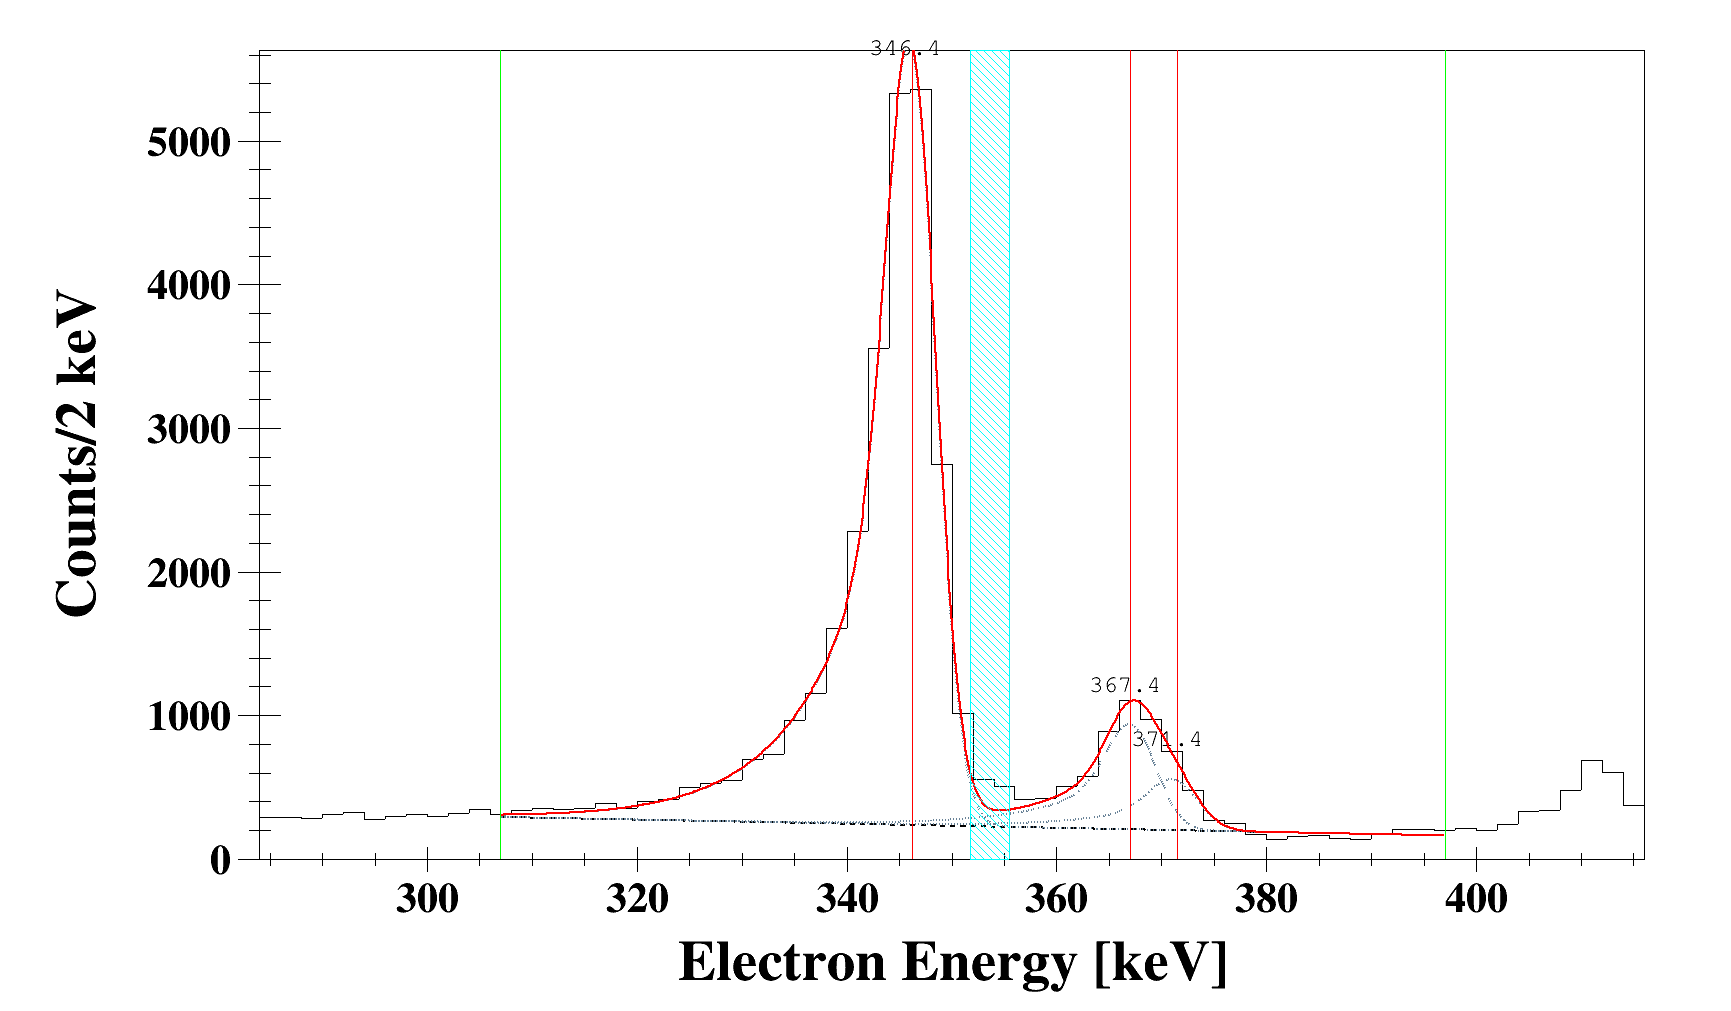
\includegraphics[width=\textwidth]{techniques_fit_example.png}
  \caption[An example of simultaneously fitting three peaks in the $\alpha$-energy gated $e^-$ data. The $K$ to $L$ peak intensity ratios are unconstrained.]{An example of simultaneously fitting three peaks in the $\alpha$-energy gated $e^-$ data. The major peak at 346.4 keV corresponds to $K$ shell electrons from the $2^+_1 \rightarrow 0^+_1$ transition in $^{110}\mathrm{Pd}$. The $L$ peak for this transition lies at 367.4 keV, while the peak at 371.4 keV was identified as belonging to a $(3^+) \rightarrow 2^+$ transition (parentheses denote a tentative multipolarity assignment), also from $^{110}\mathrm{Pd}$, with $\gamma$-ray energy of 398.6 keV. In this fit the energy separations between all peaks are fixed, but the inter-peak height ratios are not. The red vertical lines denote the peak centroids used by the fitting program, the green lines delimit the energy range considered by the fit, and the dashed blue area highlights an area of data that was excluded from the fit.}
  \label{figure: example 2 to 0 fit}
\end{figure}

There are fits for which constraining the $K$ to $L$ peak intensity ratio becomes necessary, an example of this is shown in Figure \ref{figure: example constrained fit}. The close clustering of peak structures from several identified transitions renders the use of an intensity constraint unavoidable. Hence, only a $K$ peak measurement is carried forward to the normalization procedure as an independent measurement. 

\begin{figure}[!ht]
  \centering
  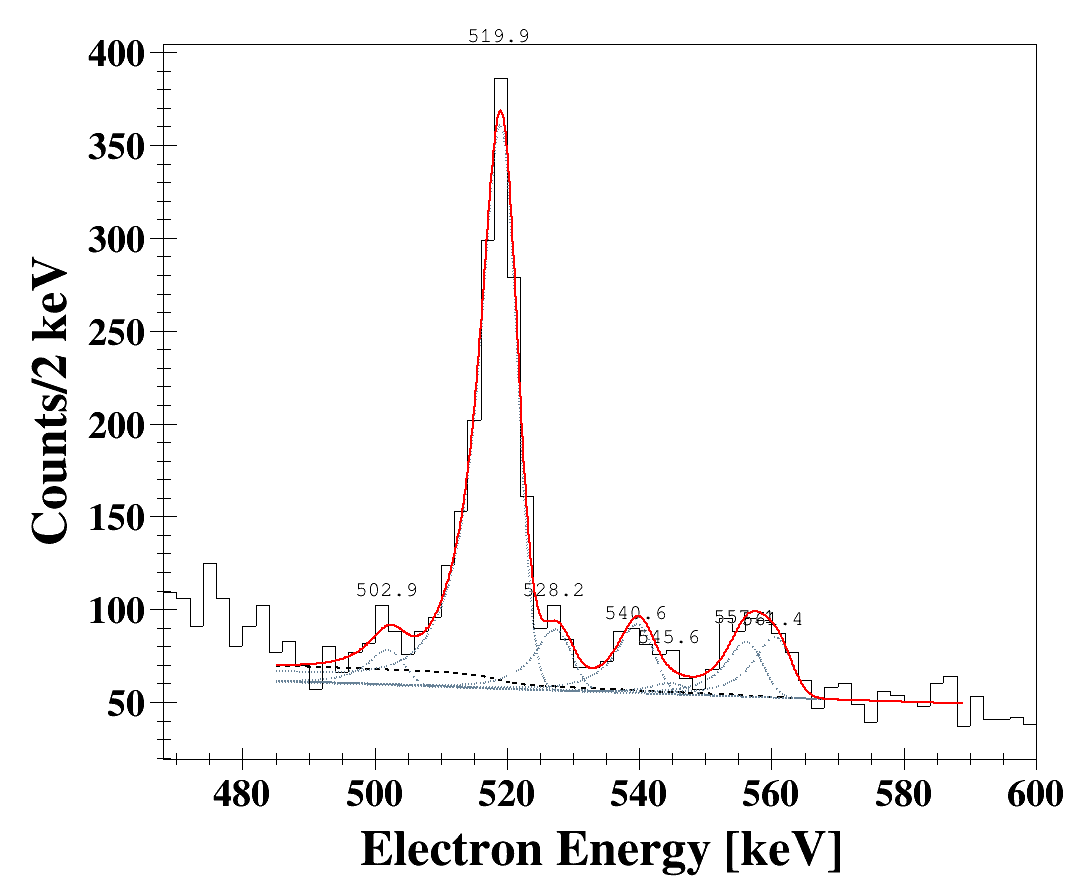
\includegraphics[width=\textwidth]{techniques_fit_constrained.png}
  \caption[An example of simultaneously fitting seven peaks in the $\alpha$-energy gated $e^-$ data. The $K$ to $L$ peak intensity ratios are constrained.]{An example of simultaneously fitting seven peaks in the $\alpha$-energy gated $e^-$ data. Here the peak at 519.9 keV is the $K$ shell peak for the $4^+_1 \rightarrow 2^+_2$ transition in $^{110}\mathrm{Pd}$. The corresponding $L$ peak is at 540.6 keV. There are several other identified transitions with peak structures present and included in the fit. The intensity ratio between the $K$ and $L$ peaks of the transitions of interest is constrained using the theoretical values from BrIcc \cite{KIBEDI2008202}.}
  \label{figure: example constrained fit}
\end{figure}

Figures \ref{figure: example 2 to 0 fit} and \ref{figure: example constrained fit} show data that is obtained by performing an energy gate on the recoiling $\alpha$ particle detected by the downstream S3 detector. Gating on an $\alpha$ particle amounts to selecting out only those $e^-$ that were detected, by SPICE, coincident in time with an $\alpha$ particle in the S3 detector. In this example a further pruning of the spectrum is achieved by gating on a specified range of $\alpha$ particle energies. This technique applies equally to the analysis of $\gamma$-ray spectra, and must be applied equivalently in form when measuring internal conversion coefficients, i.e. a direct comparison of intensities from the two types of radiated particles. 

The $\Delta E - E$ particle identification plot from the S3 detectors is shown in Figure \ref{figure: particle ID with alpha energy}. The experimental setup included multiple S3 detectors arranged in a telescope configuration that allows for the identification of particles based on their differential energy loss. The elastic peak, the highest intensity point at {\raise.17ex\hbox{$\scriptstyle\sim$}} 3600 keV total energy, corresponds predominantly to false coincidence between the elastic $\alpha$ particle beam, and the radiation from inelastic reaction products such as the Cd isotopes. Hence, two protons have been transferred to the $^{110}$Pd target, and some number of neutrons are detected by the S3. Moving along the intensity curve, upward in $\Delta E$ and leftward in $E$, inelastic, Coulomb excitation reactions exciting $^{110}$Pd to successively higher energy states are observed. The decay radiation from these states is observed in coincidence with an S3 detected $\alpha$ recoil. Nearing the end of this curving feature, the highest $\Delta E$ particles detected correspond to inelastic scattering of a high enough energy to dislodge neutrons from the target. These neutrons, and the incident $\alpha$ particle, are detected in coincidence with radiation from the nuclei $^{109}$Pd and $^{108}$Pd. The separate features, in the lower ranges of both $\Delta E$ and $E$, correspond to inelastic reactions wherein a single proton from the incident $\alpha$ particle is captured by a target nucleus, and the recoiling proton, deuteron (one proton, one neutron), or tritium (one proton, two neutrons) is detected in the S3 along with the possible free neutron products. These detections are coincident with the radiation emitted by the Ag isotopes. 

\begin{figure}[!ht]
  \centering
  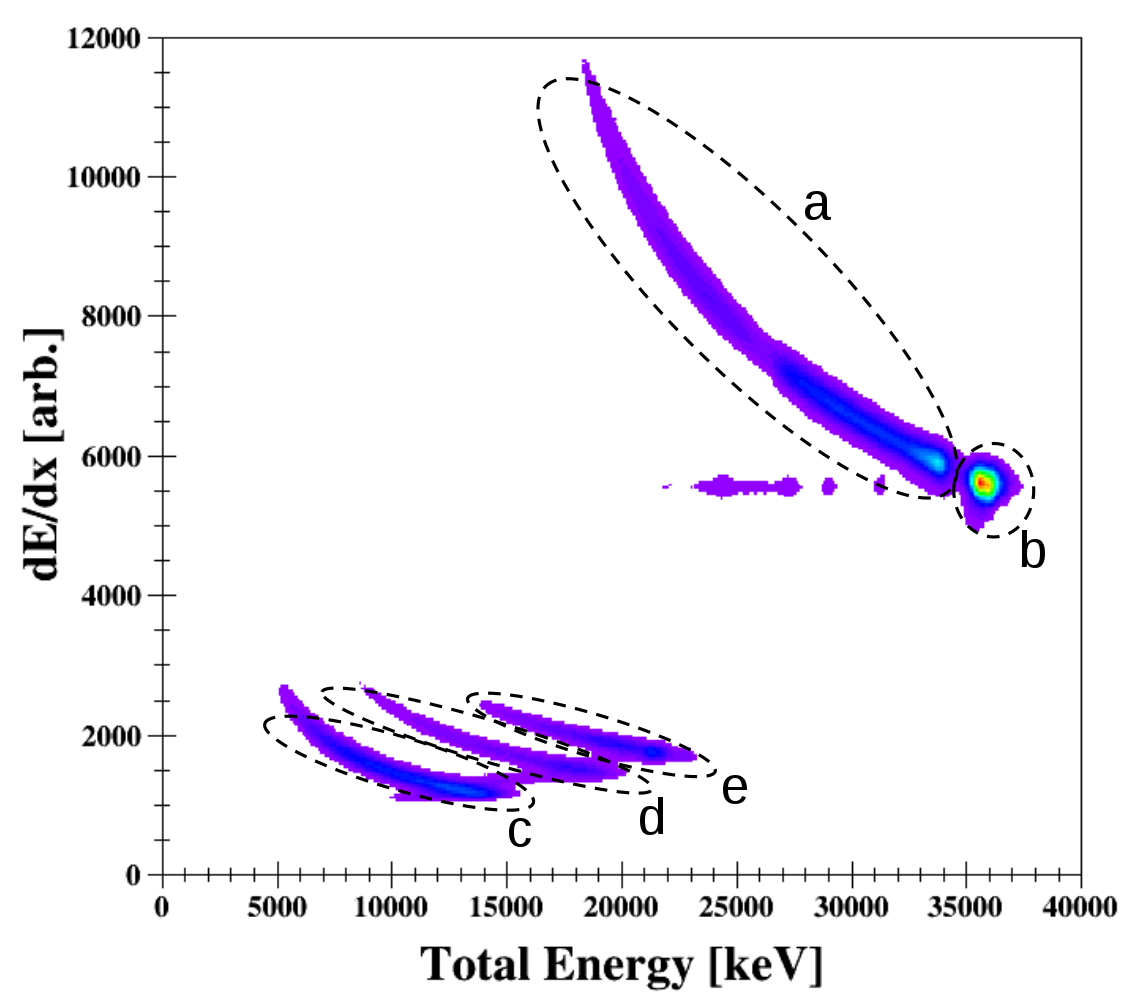
\includegraphics[width=\textwidth, height=0.84\textwidth]{techniques_particle_ID.png}
  \caption[$\Delta E - E$ particle identification plot from the S3 telescope.]{$\Delta E - E$ particle identification plot from the S3. The experimental setup included multiple S3 detectors arranged in a telescope configuration that allows for the identification of particles based on their differential energy loss: a) Inelastic, Coulomb excitation reactions, exciting $^{110}$Pd to successively higher energy states. Nearing the end of this curving feature, the highest $\Delta E$ detections are inelastic scattering $\alpha$ particles coincident with the nuclei $^{109}$Pd and $^{108}$Pd. b) The elastic peak, corresponding predominantly to random coincidence between the elastic $\alpha$ particle beam, and the radiation from inelastic reaction products such as the Cd isotopes. The separate features, c, d, and e, correspond to detected protons, deuterons, and tritons, respectively. These are inelastic reactions wherein a single proton from the incident $\alpha$ particle is captured by a target nucleus. These detections are coincident with the radiation emitted by the Ag isotopes.}
  \label{figure: particle ID with alpha energy}
\end{figure}

Gating on the energy range in detected $\alpha$ particles presented a sufficiently clean, i.e. removing enough of the unwanted transitions and background, $\gamma$-ray and $e^-$ spectra for the internal conversion coefficient analysis. All of the spectra fitting analysis was performed using an analysis package called jRootAnalysisTools, developed at TRIUMF, and built upon the ROOT data analysis framework \cite{Brun1997}.

%%%%%%%%%%%%%%%%%%%%%%%%%%%%%%%%%%%%%%%%%%%%%%%%
\section{Calibration of Detection Efficiency}
\label{sec: Calibration of Detection Efficiency}
%%%%%%%%%%%%%%%%%%%%%%%%%%%%%%%%%%%%%%%%%%%%%%%%

To be assured of accuracy of experimental data, a calibration of the SPICE detector using radioactive source data was necessary. Both before and after the experimental campaign, a radioactive $^{207}\mathrm{Bi}$ source was used in calibration. $^{207}\mathrm{Bi}$ is chosen because it has an intense, easily resolvable, internal conversion electron spectrum. The 120 individual segments of the SPICE Si(Li) detector were reviewed for there accuracy of reproducing the expected $^{207}$Bi electron spectrum. 9 channels were deemed to be ineffective, and were removed from the final data set sorted for analysis.

All of the data for the experimental analysis was sorted using a sorting program called GRSIsort, developed by the Gamma-Ray Spectroscopy at ISAC (GRSI) group \cite{GRSIsort}. 

%%%%%%%%%%%%%%%%%%%%%%%%%%%%%%%%%%%%%%%%%%%%%%%%
\section{Simulated SPICE Efficiency}
\label{sec: Simulated SPICE Efficiency}
%%%%%%%%%%%%%%%%%%%%%%%%%%%%%%%%%%%%%%%%%%%%%%%%

The TIGRESS and SPICE detectors have unique particle detection efficiencies. In order to make absolute measurements of physical events, the efficiency of the detectors must be considered. If the $\gamma$-ray and $e^-$ efficiencies were equivalent, then any error resulting from detection inefficiencies would cancel. It is the relative efficiency between the two detectors that matters. This can be seen explicitly from the way that the internal conversion coefficient is calculated

\begin{gather}
\alpha_K= \frac{A_e}{A_\gamma} \cdot \frac{\epsilon_\gamma}{\epsilon_e}
\label{equation: ICC and Efficiency}
\end{gather}

where $A_e$ and $A_\gamma$ are the measured $e^-$ and $\gamma$-ray counts. The $\gamma$-ray detection efficiency, $\epsilon_\gamma$, of TIGRESS is well characterized, via a previous efficiency calibration with $^{152}\mathrm{Eu}$, $^{133}\mathrm{Ba}$, $^{207}\mathrm{Bi}$, and $^{56}\mathrm{Co}$ sources. The $e^-$ efficiency, $\epsilon_e$, of SPICE must be determined by making measurements of internal conversion coefficients for which the transition multipolarity is known. The relative difference between these measurements and the expected values calculated by BrIcc will provide information on the efficiency of $e^-$ detection in the experiment. Additionally, the approximate shape of the SPICE efficiency curve, as it changes with incident $e^-$ energy, can be determined from simulation in Geant4. The combination of normalization from previously measured values, and an understanding of the shape of efficiency changes with energy, provides a method for calculating previously unmeasured internal conversion coefficients. 

Geant4 is a toolkit for the simulation of the passage of particles through matter \cite{Geant4}. Using a package specific to the SPICE detector, simulations at $e^-$ energies spanning the SPICE detection range were performed \cite{detectorSimulations}. The results for this simulation are shown in Figure \ref{figure: SPICE simulated efficiency}. 

% !!! The inclusion of a Geant4 viewer image with particle tracks could do

\begin{figure}[!ht]
  \centering
  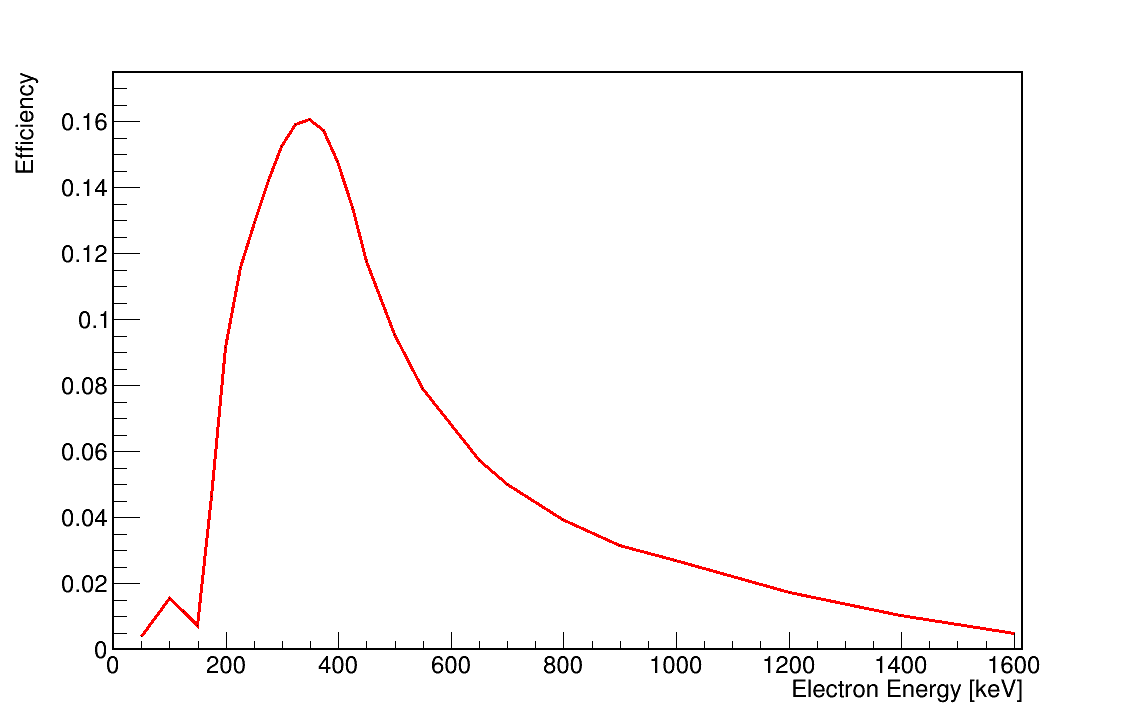
\includegraphics[width=\textwidth]{techniques_spice_simulation.png}
  \caption[A simulation of the SPICE detection efficiency using the Geant4 toolkit.]{A simulation of the SPICE detection efficiency using the Geant4 toolkit \cite{detectorSimulations,Geant4}.}
  \label{figure: SPICE simulated efficiency}
\end{figure}

% !!! The efficiency changes with beam spot characterization is could be added

% Further investigation of the resulting efficiency was undertaken. Two parameter spaces were explored in additional simulations: changing the circular area of the $e^-$ source, and moving the position of that source off of the beam line axis. The position and size of the $e^-$ source is meant to correspond to the cross-section of the incident beam particles, $\alpha$ in this experiment. The assumption of a perfectly tuned beam, i.e. directly along the axis at which the $^{110}\mathrm{Pd}$ target is placed, is investigated here. In Figures [!!!, !!!, !!!, !!!] the dimensions of the $e^-$ source is shown in conjunction with the resultant simulated SPICE efficiency curve. 

% \begin{figure}[!ht]
%   \centering
%   
\includegraphics[width=\textwidth]{placeholder.png}
%   \caption{Messing around with beam spot, several images [!!!]}
%   \label{figure: beam spot and simulated efficiency}
% \end{figure}


%%%%%%%%%%%%%%%%%%%%%%%%%%%%%%%%%%%%%%%%%%%%%%%%
\section{Determining Internal Conversion Coefficients}
\label{sec: Determining Internal Conversion Coefficients}
%%%%%%%%%%%%%%%%%%%%%%%%%%%%%%%%%%%%%%%%%%%%%%%%

For each observed transition, the number of counts in $e^-$ and $\gamma$-ray spectra is measured, and Equation (\ref{equation: ICC and Efficiency}) was used to calculate an absolute internal conversion coefficient.

The $\gamma$-ray detection efficiency, $\epsilon_\gamma$ is taken from the previously calculated efficiency curve for TIGRESS. The $e^-$ detection efficiency of SPICE was determined by using normalization transitions in order to interpolate the detector efficiency for transitions of interest. Figure \ref{figure: SPICE efficiency normalization with ICC measurements} plots the calculated efficiency and $K$ shell $e^-$ energy for the normalization transitions used, along with an exponential scaling of the simulated SPICE efficiency curve described in Section \ref{sec: Simulated SPICE Efficiency}. The scaling amounts to fitting the following function to the measured internal conversion coefficient data:

\begin{gather}
f(x) =  \epsilon_e(x) \cdot p_1 \cdot e^{\frac{-x}{p_0}} \cdot
\label{equation: exponential scaling}
\end{gather}

where $p_1$ and $p_0$ are parameters to be fit, the variable $x$ stands in for $e^-$ energy, and $\epsilon_e(x)$ is the simulated SPICE efficiency curve. The normalization transitions used are listed in Table \ref{table:norm_icc}.

\begin{figure}[!ht]
  \centering 
  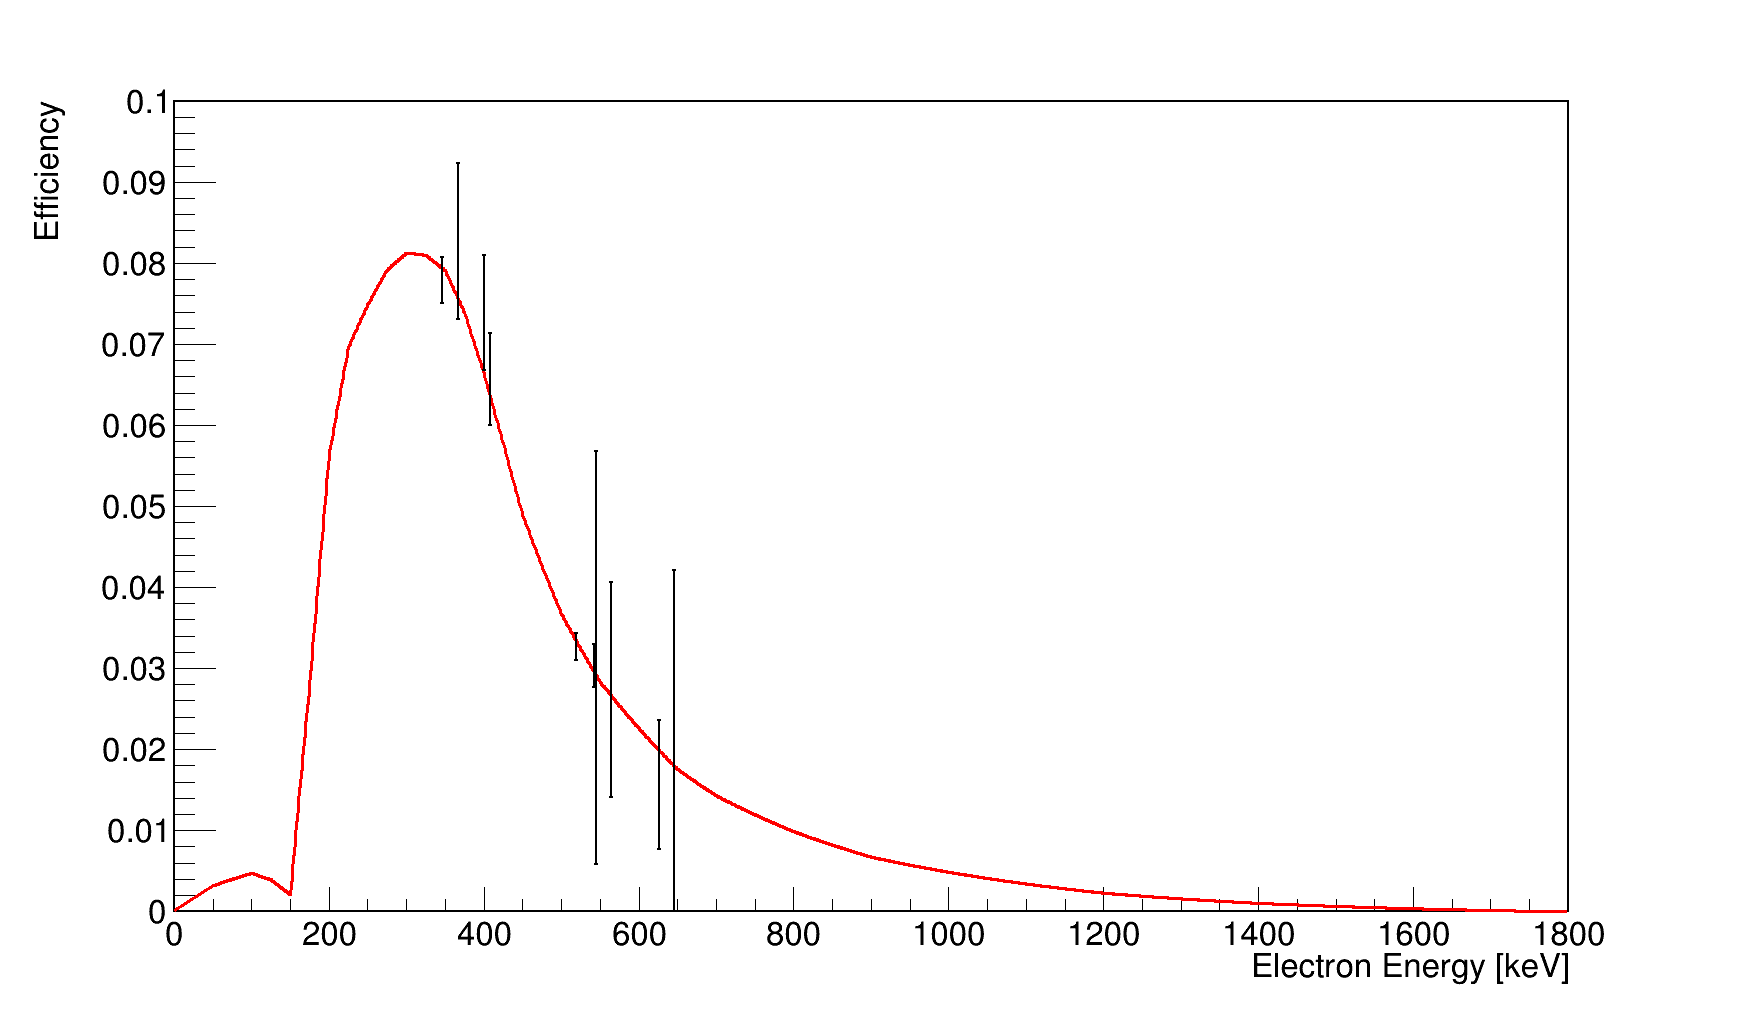
\includegraphics[width=\textwidth]{techniques_icc_scaled.png}
  \caption[The efficiency values and $K$ $e^-$ peak energies for several transitions are plotted and fit by an exponential scaling of the simulated SPICE efficiency curve.]{The efficiency values and $K$ $e^-$ peak energies for several transitions are plotted. The red curve represents the simulated SPICE efficiency curve, scaled by the fitted exponential function outlined in Equation (\ref{equation: exponential scaling}). The measurements used for this normalization routine are given in Table \ref{table:norm_icc}.}
  \label{figure: SPICE efficiency normalization with ICC measurements}
\end{figure}

% !!! When listing the spin assignments for states in this table, I've run into a question about dealing with tentative assignment. In the case of the highlighted transition from 109Pd, there is a lower energy state that is tentatively assigned as (7/2^+). Do I label the state here as the 'second' 7/2+ state with a '2' subscript? Sometimes only the parity or the spin are individually tentative. My approach has been to just leave off the numeric subscript whenever I encounter such ambiguity. 

\begin{sidewaystable}
  \begin{center}
    \begin{tabular}{|l|l l l|l l|l l|} 
     \hline
     & Transition & $E_\gamma \ [\mathrm{keV}]$ & Multipolarity & $\alpha_\mathrm{exp}(K) \times 10^3$ & $\alpha_\mathrm{exp}(L) \times 10^3$ &	$\epsilon_e (K)$ [\%]	& $\epsilon_e (L)$ [\%]\\  
     \hline
     $^{109}\mathrm{Pd}$	& $7/2^+ \rightarrow 5/2^+$	& 426.135	& $M1$	& 5.91(56)	& ---	& 7.39(71)	& --- \\
     						& $7/2^+ \rightarrow 5/2^+$	& 433.552	& $M1$	& 5.06(43)	& ---	& 6.57(57)	& --- \\
     $^{110}\mathrm{Pd}$	& $2_1^+ \rightarrow 0_1^+$ & 373.8  	& $E2$	& 10.27(33)	& 1.46(18)		& 7.78(28)	& 8.27(97)	  \\  
                         	& $4_1^+ \rightarrow 2_1^+$ & 547.04  	& $E2$	& 1.60(8)	& ---	& 3.27(17)	& ---  \\
                            & $0_2^+ \rightarrow 2_1^+$ & 572.89  	& $[E2]$& 1.4(11)	& ---	& 3.1(25)	& ---  \\
                            & $6_1^+ \rightarrow 4_1^+$ & 653.1  	& $[E2]$& 0.51(26)	& 0.04(12)		& 1.57(79)	& 1.1(31)	  \\  
     $^{111}\mathrm{Cd}$	& $15/2^- \rightarrow 11/2^-$ & 571.72 	& $E2$	& 1.48(13)	& 0.17(8)		& 3.03(27)	& 2.7(13)	  \\     
     \hline
    \end{tabular}
  \end{center}
  \caption[Table of normalization transitions used in determining $e^-$ detection efficiencies for internal conversion coefficient measurements.]{Table of normalization transitions used in determining $e^-$ detection efficiencies for internal conversion coefficient measurements. Square parentheses indicate a tentative multipolarity assignment.}
  \label{table:norm_icc}
\end{sidewaystable}

Since these are transitions of known multipolarity, the efficiency values for normalization are being calculated via the following relationship:

\begin{gather}
\epsilon_e= \frac{\alpha_\mathrm{exp}}{\alpha_\mathrm{BrIcc}} \cdot \epsilon_\gamma
\label{equation: Electron efficiency normalization}
\end{gather}

where $\alpha_\mathrm{BrIcc}$ is the theoretically calculated internal conversion coefficient from BrIcc \cite{KIBEDI2008202}.

%%%%%%%%%%%%%%%%%%%%%%%%%%%%%%%%%%%%%%%%%%%%%%%%
\section{Determining $E0$ Transition Strengths} \label{sec:Determining E0 Transition Strengths}
%%%%%%%%%%%%%%%%%%%%%%%%%%%%%%%%%%%%%%%%%%%%%%%%

Using the conversion coefficients determined in this experiment, along with previously measured experimental values such as the mixing ratio, $\delta(E2/M1)$, the $\rho^2(E0)$ value can be determined from \cite{Kibedi2005}

\begin{gather}
\rho^2(E0) = \frac{1}{\Omega_K(E0) \cdot \tau_K(E0)}
\label{equation: E0 strength via partial lifetimes}
\end{gather}

where $\Omega$ is the electronic factor obtained from BrIcc \cite{KIBEDI2008202} and $\tau(E0)$ is the partial mean lifetime of the $E0$ transition. The subscript $K$ denotes that the $E0$ strength is calculated for $K$ shell internal electron conversion. The partial mean lifetime, $\tau(E0)$, is calculated via

\begin{gather}
\tau(E0) = \frac{\Sigma \lambda_r}{\lambda_r(E0)} \cdot \tau
\label{equation: partial lifetime from relative decay constants}
\end{gather}

where $\tau = T_{1/2}/\ln(2)$ and $\lambda_r$ is the relative decay constant which is specific to each available decay mode from the parent state \cite{KraneText}. Hence the summation over all decay modes is performed in order to quantify the fractional value of the $E0$ lifetime relative to all other modes. An example is shown in Table \ref{table: inputs to the partial lifetime calculation of E0 strength} for the $2_2^+ \rightarrow 2_1^+$ transition in $^{110}\mathrm{Pd}$.

\begin{table}
  \begin{center}
    \begin{tabular}{|l|l|l|l|l|l|} 
     \hline
     $i$& Transition 					& Multipolarity & Mode 					& Method 					& $\lambda_r$ 			\\  
     \hline
     0	& A$(2_2^+ \rightarrow 2_1^+)$	& $E2$			& $\gamma$				& Set to 1					& 1						\\ 
     1	&								& 				& $e^-$					& $i_0 \cdot \alpha_K(E2)$	& $7.56 \times 10^{-3}$	\\ 
     2	&								& $M1$			& $\gamma$				& $i_0 / \delta^2$			& $4.72 \times 10^{-2}$	\\ 
     3	&								& 				& $e^-$					& $i_2 \cdot \alpha_K(M1)$	& $3.14 \times 10^{-4}$	\\ 
     4	&								& $E0$			& $e^-$					& $i_1 \cdot q_K^2$			& $-1.10 \times 10^{-4}$	\\ 
     5	& B$(2_2^+ \rightarrow 0_1^+)$	& 				& all					& 							& 0.37					\\
     \hline
     	&	A							&				& $\lambda_r(E0)$		& $i_4$ 					& $-1.10 \times 10^{-4}$	\\
    	&	A \& B						&				& $\Sigma \lambda_r$	&							& 1.42					\\
     \hline
    \end{tabular}
  \end{center}
  \caption[The calculation of $\lambda_r$ for each possible decay mode from the $2^+_2$ state in $^{110}$Pd.]{The calculation of $\lambda_r$ for each possible decay mode from the $2^+_2$ state in $^{110}$Pd. The errors are excluded in this table but are determined for the final value with a Monte Carlo method.}
  \label{table: inputs to the partial lifetime calculation of E0 strength}
\end{table}

The input $\delta(E2/M1)$ value carries a large, asymmetric uncertainty value. In a traditional approach to error propagation, a series of summations of real and fractional measurement error, in quadrature, would yield a final error estimate for $\rho^2(E0)$. However this approach is not applicable in instances of asymmetric error on inputs, and will yield an incorrect result. As such, the final value in this work is determined through a Monte Carlo method.

In the Monte Carlo method, each experimental value used as an input is assumed to be a normal distribution with a mean and width given by ($\mu, \sigma $). A simulation is performed, in which each event results in a calculation of $\rho^2(E0)$ using input values chosen at random from each distribution of ($\mu, \sigma$). These calculations, each instance being an iteration of Equation (\ref{equation: E0 strength via partial lifetimes}), fill a distribution of $\rho^2(E0)$ values. An example distribution for the $2_2^+ \rightarrow 2_1^+$ transition in $^{110}\mathrm{Pd}$ is shown in Figure \ref{figure: Monte Carlo distribution}.

\begin{figure}[!ht]
  \centering
  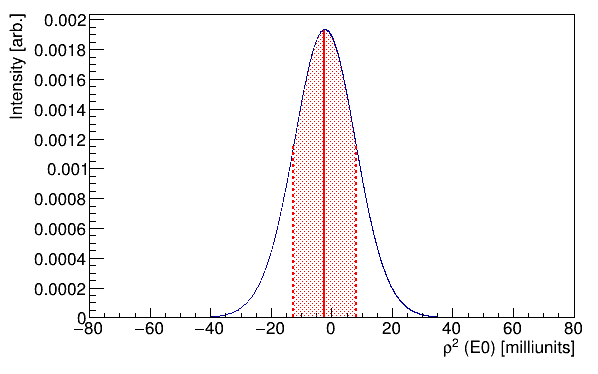
\includegraphics[width=\textwidth]{techniques_monte_carlo.png}
  \caption[An example distribution of $\rho^2(E0)$for the $2_2^+ \rightarrow 2_1^+$ transition in $^{110}\mathrm{Pd}$, produced by the Monte Carlo method.]{An example distribution of $\rho^2(E0)$for the $2_2^+ \rightarrow 2_1^+$ transition in $^{110}\mathrm{Pd}$, produced by the Monte Carlo method. The solid red line is the mean of the distribution and the shaded error is the $68\%$ confidence limit, or 1$\sigma$.}
  \label{figure: Monte Carlo distribution}
\end{figure}

In the example shown in Figure \ref{figure: Monte Carlo distribution} the mean of the distribution is in the unphysical ($< \ 0$) region. This result constitutes an effective measurement of zero, indicating a negligible $E0$ component to the transition. The negative, unphysical result is interpreted as a byproduct of measurement uncertainty and statistical methodology. An additional statistical finesse is required in order to interpret this result and extract a measurement. 

In a Bayesian statistical model, the approach of taking the product of this distribution with a `prior' distribution would be used. The prior distribution is a chosen function that represents all \textit{a priori} knowledge about the expected value. In this case, where $\rho^2(E0)$ is defined to be non-negative, a distribution that is constant for $x>0$, and zero for $ x \leq 0$ could be chosen. However this is considered to be an arbitrary solution \cite{GregoryText}. The alternative is the Neyman construction using the Feldman-Cousins ordering principle \cite{JamesText}. In this method, the distribution is used to determine the upper and lower limit in each true value of $\rho^2(E0)$, i.e. each y-slice in Figure \ref{figure: Monte Carlo distribution}. This construction assumes that the experimentally measured value of $\rho^2(E0)$ is representative of the unique experimental ensemble used to achieve the measurement. Implied is the existence of a distribution of experimental ensembles that could have been used to make the measurement, ensembles varying in their detector properties and other such systematics. The Neyman construction uses a frequentist statistical approach and yields confidence intervals describing the likelihood of the true $\rho^2(E0)$, as it exists in nature, coinciding with the measurement carried out by our experimental ensemble.

The Feldman-Cousins ordering principle is an alternative way of determining the confidence limits i.e. instead of simply rearranging the distribution from maximum to minimum, a separate ratio is calculated from \cite{JamesText}

\begin{gather}
R = \frac{P(x\rvert \mu)}{P(x\rvert \mu_\mathrm{best})}
\label{eq:feldman cousins}
\end{gather}

where $\mu_\mathrm{best}$ is the most likely value of $\mu$ in the physical (i.e. $x > 0$) region. The distribution is then ordered from the highest value of $R$ to the lowest and counted again until 68\% of the distribution is obtained. This method essentially adjusts coverage of the confidence region to remain in the physically allowed area. Using the distribution of Figure \ref{figure: Monte Carlo distribution}, the Feldman-Cousins ordering principle is used to determine the confidence limits for the Neyman construction in Figure \ref{figure: Neyman construction}. As the measured mean value is -2.325, a dashed line is drawn to determine the upper limit of +8.31. 

\begin{figure}[!ht]
  \centering
  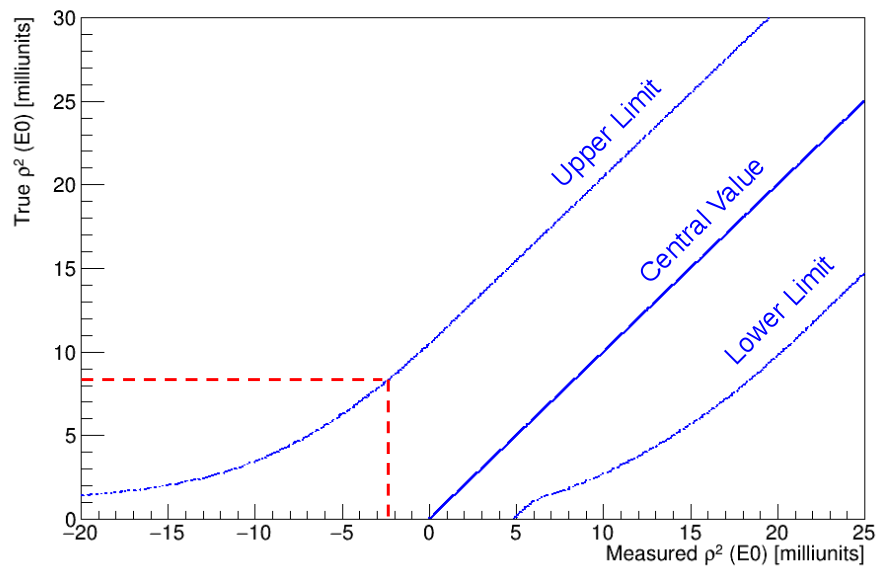
\includegraphics[width=\textwidth]{techniques_neyman.png}
  \caption[An example of the Neyman Construction produced using the distribution of Figure \ref{figure: Monte Carlo distribution}.]{An example of the Neyman Construction produced using the distribution of Figure \ref{figure: Monte Carlo distribution}. The measured mean value of the distribution was -2.325, a dashed line is drawn to determine the upper confidence limit of +8.31.}
  \label{figure: Neyman construction}
\end{figure}


\endinput

Any text after an \endinput is ignored.
You could put scraps here or things in progress.

%%%%%%%%%%%%%%%%%%%%%%%%%%%%%%%%%%%%%%%%%%%%%%
JTS from Paper
%%%%%%%%%%%%%%%%%%%%%%%%%%%%%%%%%%%%%%%%%%%%%%

{\it Experimental Details -}
% Beamtime was June 2016. TIGRESS elogs 14417 to 14687.
A beam of 35.6\,MeV alpha particles with a typical intensity of 120\,ppA was delivered by the TRIUMF-ISAC-II superconducting linear accelerator to the TIGRESS spectrometer. The beam was incident on a self-supporting $^{110}$Pd target of 1.6\,mg/cm$^2$ with a 97.61\% isotopic enrichment. The target was positioned 8\,mm upstream of the nominal center of the TIGRESS spectrometer.
Two micron S3 silicon detectors of 140\,$\mu$m and 1000\,$\mu$m thickness were located downstream in a $\Delta E-E$ telescope configuration to detect and identify charged particles. Twelve of the TIGRESS high-purity germanium (HPGe) clover detectors were positioned around the target location to detect $\gamma$ rays. Four clovers were located at 45$^{\circ}$ with respect to the beam axis, and the remaining eight at 90$^{\circ}$. Each clover was fully Compton suppressed and positioned at a target-to-detector distance of 14.5\,cm in the `Optimized peak-to-total' configuration of the TIGRESS spectrometer \cite{Hackman14}.

The spectrometer for internal conversion electrons (SPICE) detector was used to detect internal conversion electrons emitted from excited states populated in the reaction. The main detector of SPICE is a 6.1\,mm thick lithium-drifted silicon (Si(Li)) detector shielded by a photon shield from direct sight of the target. A magnetic lens formed of rare-earth permanent magnets collects and directs internal conversion electrons around the photon shield into the Si(Li) detector. The annular detector with inner and outer radii of 1 and 10\,cm is segmented into 120 individual segments arranged with 12 azimuthal sectors and 10 rings.

The detector signals were processed by the TIGRESS data acquisition system \cite{Martin08}. Data were collected when one of three hardware coincidence triggers between detector types was satisfied; [Si(Li) + S3], OR [Ge + S3] OR [Si(Li) + Ge]. In the case of S3 a pre-trigger coincidence between the delta-E and E detectors was required.

%%%%%%%%%%%%%%%%%%%%%%%%%%%%%%%%%%%%%%%%%%%%%%
Daniel's report
%%%%%%%%%%%%%%%%%%%%%%%%%%%%%%%%%%%%%%%%%%%%%%

The TRIUMF-ISAC Gamma-Ray Escape-Suppressed Spectrometer (TIGRESS) is a gamma- ray detector array situated at TRIUMF, Canada’s national laboratory for particle and nuclear physics. TIGRESS consists of up to 16 gamma-ray detectors; each detector contains 4 high- purity germanium (HPGe) crystals, which can provide high-resolution measurements of the detected gamma-ray energies. The HPGe detectors are highly segmented, which allows de- termination of the gamma-ray interaction location. Because of the high velocity of the beam, gamma-ray energy peaks are Doppler-shifted and broadened in an angle-dependent manner, and this position sensitivity allows the effect to be corrected.
When a gamma ray strikes the detector, there is a chance that it will scatter off the crystal and not deposit its full energy (known as Compton scattering). If a gamma ray scatters into an adjacent HPGe crystal, TIGRESS can add the partial energies of each hit and reconstruct the gamma-ray energy. The HPGe detectors are surrounded by scintillator shields made from bismuth germanate (BGO) and cesium iodide (CsI) crystals. These shields can detect gamma rays that escape the HPGe crystals without depositing their full energy, and then reject those gamma-rays from the collected HPGe spectrum. These techniques increase the peak-to-total ratio of the spectrum [4].
TIGRESS can be equipped with ancillary detectors, including SPICE, the Spec- trometer for Internal Conversion Electrons. When nuclei de-excite, there is a chance that
3
rather than emitting a gamma-ray, an electron is instead ejected from the atom. These electrons may be measured with SPICE, providing information about the multipolarity of different transitions. A primary aim is to measure transitions between two 0+ states, and determine electric monopole (E0) transition strengths [5]. SPICE may be equipped with an annular silicon detector positioned downstream of the target that can detect recoiling nuclei (called an "S3"), divided into 24 rings and 32 segments, allowing determination of both the angle θ and the angle φ of the recoiling particles. The recoil detector has the energy resolution to distinguish between recoils of different species, so more information about the kinematics of individual reactions can be obtained. Figure 1 shows the TIGRESS array and SPICE.
%% The following is a directive for TeXShop to indicate the main file
%%!TEX root = diss.tex

%%%%%%%%%%%%%%%%%%%%%%%%%%%%%%%%%%%%%%%%
\chapter{Results and Discussion}
\label{ch:ResultsandDiscussion}
%%%%%%%%%%%%%%%%%%%%%%%%%%%%%%%%%%%%%%%%

The results of the experimental measurements are presented in this chapter. In Section \ref{sec: Determining Internal Conversion Coefficients} it was shown how previously unmeasured internal conversion coefficients may be determined. These new measurements are detailed in Section \ref{sec: Measured E0 Transition Strengths}. For the $2^+_2 \rightarrow 2^+_1$ transition in $^{110}\mathrm{Pd}$, a newly measured internal conversion coefficient was combined with other experimental data to calculate the $E0$ transition strength. In Section \ref{sec: Measured E0 Transition Strengths} this result is presented within the context of similar measurements performed in other isotopes of Pd. 

%%%%%%%%%%%%%%%%%%%%%%%%%%%%%%%%%%%%%%%%
\section{Measured Internal Conversion Coefficients}
\label{sec: Measured Internal Conversion Coefficients}
%%%%%%%%%%%%%%%%%%%%%%%%%%%%%%%%%%%%%%%%

The measured internal conversion coefficients (for the $K$ shell) are presented in Table \ref{table:measured_ICC} in conjunction with theoretical values from BrIcc \cite{KIBEDI2008202}. Comparison with the BrIcc values shows that certain multipolarities are less probable than others for the measured transitions. However, the measurements do not provide a definitive argument as to the exact multipolarities of any of the measured transitions.

\begin{table}
  \begin{center}
    \begin{tabular}{|l|l l|l|l l l l|} 
     \hline
     & Transition & $E_\gamma \ [\mathrm{keV}]$ & $\alpha_\mathrm{exp}(K)$ & \multicolumn{4}{c|}{BrIcc $\alpha(K)$} \\
     & \multicolumn{2}{c|}{} &  										& $E1$		& $M1$		& $E2$		& $M2$		\\  
     \hline 
     $^{109}\mathrm{Pd}$ & $1/2, 3/2 \rightarrow 5/2^-$ 			& 530.202 	& 7(2)	& 1.44(2)	& 4.24(6)	& 4.38(7)	& 13.3(2)	\\ 
     \hline 
     $^{110}\mathrm{Pd}$ & $(3^+) \rightarrow 2^+_2$ 				& 398.6   	& 14(3) & 2.90(4)	& 8.5(1) 	& 10.2(2) 	& 31.0(5) 	\\  
                         & $(6^+) \rightarrow 4^+_2$ 				& 588.8   	& 5(2) 	& 1.13(2) 	& 3.31(5) 	& 3.27(5) 	& 9.9(1)	\\ 
                         & $(4^+) \rightarrow (3^+)$ 				& 687.7   	& 4(2) 	& 0.81(1)	& 2.30(4) 	& 2.17(3)	& 6.41(9) 	\\    
     \hline 
     $^{111}\mathrm{Ag}$ & $11/2^{(+)} \rightarrow 9/2^+_1$ 		& 575.1 	& 5(3)& 1.27(2)	& 3.81(6)	& 3.68(6)	& 11.5(2)	\\  
                         & $11/2^+, 13/2_1^+ \rightarrow 9/2_1^+$ 	& 694.19    & 5(1)& 0.84(1) 	& 2.45(4) 	& 2.24(4) 	& 6.8(1)	\\  
     \hline
    \end{tabular}
  \end{center}
  \caption[Measured internal conversion coefficients for the $K$ electron shell, $\alpha_\mathrm{exp}(K)$, compared to the theoretically calculated values from BrIcc \cite{KIBEDI2008202}.]{Measured internal conversion coefficients for the $K$ electron shell, $\alpha_\mathrm{exp}(K)$, compared to the theoretically calculated values from BrIcc \cite{KIBEDI2008202}. All internal conversion coefficient values are given in milliunits. Calculated values from BrIcc are denoted by the multipolarity assumed for the transition. $E_\gamma$ is the transition energy. The enclosure of a nuclear level's spin and/or parity assignment, such as $(3^+)$, indicates a tentative assignment.}
  \label{table:measured_ICC}
\end{table}

Two measurements were made of $K$ shell internal conversion coefficients for mixed transitions. These two results are presented in Table \ref{table:measured_mixed_ICC}.

\begin{table}
  \begin{center}
    \begin{tabular}{|l|l l|l|l|l l l|} 
     \hline
     & Transition & $E_\gamma \ [\mathrm{keV}]$ &$\delta(E2/M1)$& $\alpha_\mathrm{exp}(K)$ & \multicolumn{3}{c|}{BrIcc $\alpha(K)$} \\
     &  \multicolumn{2}{c|}{}	& 		& 			& $E2$		& $M1$		& $(E2/M1)$	\\  
     \hline 
     $^{110}\mathrm{Pd}$	& $2_2^+ \rightarrow 2_1^+$ & 439.76 & $-4.6^{+1.9}_{-1.2}$	& 7.4(5)	& 7.6(1) 	& 6.6(1)	& 7.5(1)	\\  
                         	& $4_2^+ \rightarrow 4_1^+$ & 477.8  & Unmeasured			& 7(3)		& 5.9(1) 	& 5.4(1)	& 5.7(3)	\\   
     \hline
    \end{tabular}
  \end{center}
  \caption[Measured internal conversion coefficients for known mixed transitions, $\alpha_K$ (for the K electron shell), compared to the theoretically calculated values from BrIcc \cite{KIBEDI2008202}.]{Measured internal conversion coefficients for known mixed transitions, $\alpha_K$ (for the K electron shell), compared to the theoretically calculated values from BrIcc \cite{KIBEDI2008202}. All internal conversion coefficient values are given in milliunits. For the $4_2^+ \rightarrow 4_1^+$ transition in $^{110}\mathrm{Pd}$ the BrIcc default value of 1.00 for $E2/M1$ mixing is used. $E_\gamma$ is the transition energy.}
  \label{table:measured_mixed_ICC}
\end{table}

The measured internal conversion coefficient for the $2_2^+ \rightarrow 2_1^+$ transition is consistent with the prediction from BrIcc. There is little that can be said about the measured internal conversion coefficient for the $4_2^+ \rightarrow 4_1^+$ transition, as no mixing ratio has been measured. 

%%%%%%%%%%%%%%%%%%%%%%%%%%%%%%%%%%%%%%%%
\section{Measured $E0$ Transition Strengths}
\label{sec: Measured E0 Transition Strengths}
%%%%%%%%%%%%%%%%%%%%%%%%%%%%%%%%%%%%%%%%

Using the experimental values of the internal conversion coefficients measured in this work, in combination with other experimental and theoretical values from literature \cite{KIBEDI2008202,ENSDF110Pd}, the $E0$ transitions strengths were evaluated for the $2_2^+ \rightarrow 2_1^+$ transition in $^{110}\mathrm{Pd}$. In Table \ref{table: Comparing E0 Strengths of Pd Nuclei}, the measurement resulting from the Monte Carlo analysis and Neyman construction is given in comparison to other $\rho^2(E0)$ measurements in the Pd nuclei. For transitions where there are two existing measurements of the $(E2/M1)$ mixing ratios, both values and their corresponding $\rho^2(E0)$ measurements are given. The Monte Carlo error analysis was carried out with $10^8$ simulation events. The bin size of the resulting $\rho^2(E0)$ distribution was 0.05 milliunits. In the construction of the Neyman plots (using the Feldman-Cousins ordering principle), each vertical row of the `true' mean value was calculated every 0.001 milliunits.

Additionally, an upper limit has been given for the $\rho^2(E0)$ value in the $4^+_2 \rightarrow 4^+_1$ transition of $^{110}$Pd. A maximal value for the mixing ratio has been assumed for this calculation, implying a transition that has a negligible $M1$ component. The calculation of this limit followed the same Monte Carlo and Neyman methodology as detailed for the $2^+_2 \rightarrow 2^+_1$ transition. 

\begin{sidewaystable}
\begin{center}
\begin{tabular}{|l|l l l l|l l l|} 
\hline
& Transition & $E_\gamma \ [\mathrm{keV}]$ & $\mathrm{T}_{1/2} \  [\mathrm{ps}]$ & $\delta(E2/M1)$ & $\alpha_\mathrm{exp}(K) \times 10^3 $ & $q^2_K(E0/E2)$ & $\rho^2(E0) \times 10^3$\\
\hline
$^{102}\mathrm{Pd}$&$0_2^+\rightarrow 0_1^+$&1592.6 &$14.5(4)\times 10^3$	&&&$>2$        & $4.0(15)$\\
                   &$0_3^+\rightarrow 0_1^+$&1658.1 &$0.87(22)$  			&&&$<0.0014$ & $<0.2$\\
\hline
$^{104}\mathrm{Pd}$&$0_2^+\rightarrow 0_1^+$&1333.6 &$5.2(5)$    			&&&$0.12(6)$	& $6(4)$\\ 
\hline 


$^{106}\mathrm{Pd}$&$0_2^+\rightarrow 0_1^+$&1133.7	&$5.813)$ &&&& $14(4)$\\
                   &$2_3^+\rightarrow 2_1^+$&1562.2	&$1.3(2)$  & $+0.24(1)$	&$1.12(15)$	&& $34(22)$\\   
                   &						 &	   	&									&&$1.56(24)$&& $97(39)$\\                   
                   &$0_3^+\rightarrow 0_1^+$&1194.5	&$2.8(5)$    			&& 					 		&& $<3$\\                  
                   &$2_4^+\rightarrow 2_1^+$&1397.4	&$1.1^{+10}_{-2}$					&$1.32^{+11}_{-25}$			&$0.68(9)$ 	&& $21^{+10}_{-21}$\\                   
                   &						&	   	&									&$0.17^{+4}_{-1}$  			&&& $18^{+10}_{-18}$\\                   
                   &$4_2^+\rightarrow 4_1^+$&703.11	&$0.50^{+24}_{-2}$    				&$0.66^{+48}_{-33}$			&$1.46(26)$	&& $96^{+43}_{-61}$\\                   
\hline
$^{108}\mathrm{Pd}$&$0_2^+\rightarrow 0_1^+$&1052.8	&$4.0(4)$    			&&&$<0.02$              	& $<3$\\
\hline 
$^{110}\mathrm{Pd}$&$0_2^+\rightarrow 0_1^+$&946.7 	&$7.9(7)$    			&&&$0.034(6)$ 	& $4.0(8)$  	\\
                   &$2_2^+\rightarrow 2_1^+$&439.76	&$17.7(8)$   			& $-4.6^{+1.9}_{-1.2}$  	& $7(1)^\dagger$  	& --- & $<9^\dagger$\\
                   &$4_2^+\rightarrow 4_1^+$&477.8	&$5.1(6)$    			& Unmeasured            	& $7(3)^\dagger$ & --- & $<129^\dagger$\\
\hline
\end{tabular}
\end{center}
\caption[A comparison of $E0$ transition measurements across the Pd nuclei. New measurements resulting from this work are highlighted.]{A comparison of $E0$ transition measurements across the Pd nuclei. In the nucleus $^{106}$Pd, multiple $\rho^2(E0)$ measurements have been made, and listed here, for cases where there are differing published values of $\delta(E2/M1)$ or $\alpha_\mathrm{exp}(K)$. The half-life, $T_{1/2}$, values given are for the transition parent state. The determination of a limit on $\rho^2(E0)$ for the $2_2^+ \rightarrow 2_1^+$ transition in $^{110}\mathrm{Pd}$ is consistent with the expectation of little to no shape mixing. The magnitude of the limit is consistent with that of other Pd isotopes \cite{Peters2016,Kibedi2005}. The $\rho^2(E0)$ limit determined on the $4^+_2\rightarrow4^+_1$ assumes a maximal value for the unmeasured $\delta(E2/M1)$, hence a negligible $M1$ component. $^\dagger$This work.} 
\label{table: Comparing E0 Strengths of Pd Nuclei}
\end{sidewaystable}

The measured $\rho^2(E0)$ limit for the $2_2^+ \rightarrow 2_1^+$ transition in $^{110}$Pd is consistent with the expectation of there being negligible mixing between these two intrinsic excitation bands. In comparing to the other Pd nuclei for which published measurements exist, the small magnitude of the limit appears to be consistent with the $\rho^2(E0)$ values. For the $4^+_2 \rightarrow 2^+_1$ transition in $^{110}$Pd, the lack of a measured mixing ratio yields a relatively inexact upper bound value of $<129$. 

\endinput

Any text after an \endinput is ignored.
You could put scraps here or things in progress.

% !!! A version of the final table where measurements are more rigorously cited. Simplifying things as much as possible for the draft.

\begin{sidewaystable}
\begin{center}
\begin{tabular}{|l|l l l l|l l l|} 
\hline
& Transition & $E_\gamma \ [\mathrm{keV}]$ & $\mathrm{T}_{1/2} [ps]$ & $\delta(E2/M1)$ & $\alpha_K \times 10^3 $ & $q^2_K(E0/E2)$ & $\rho^2(E0) \times 10^3$\\
\hline
$^{102}\mathrm{Pd}$&$0_2^+\rightarrow 0_1^+$&1592.6 &$14.54})\times 10^3$	&&&$>2$\textsuperscript{a}        & $4.015})$\textsuperscript{a}\\
                   &$0_3^+\rightarrow 0_1^+$&1658.1 &$0.8722})$  			&&&$<0.0014$\textsuperscript{a} & $<0.2$\textsuperscript{a}\\
\hline
$^{104}\mathrm{Pd}$&$0_2^+\rightarrow 0_1^+$&1333.6 &$5.25})$    			&&&$0.126})$\textsuperscript{a}	& $64})$\textsuperscript{a}\\ 
\hline 


$^{106}\mathrm{Pd}$&$0_2^+\rightarrow 0_1^+$&1133.7	&$5.813})$ &&&& $144})$\textsuperscript{a}\\
                   &$2_3^+\rightarrow 2_1^+$&1562.2	&$1.32})$  & $+0.241})$\textsuperscript{b}	&$1.1215})$\textsuperscript{c}	&& $3422})$\textsuperscript{d}\\   
                   &						 &	   	&									&&$1.5624})$\textsuperscript{e}&& $9739})$\textsuperscript{d}\\                   
                   &$0_3^+\rightarrow 0_1^+$&1194.5	&$2.85})$    			&& 					 		&& $<3$\textsuperscript{d}\\                  
                   &$2_4^+\rightarrow 2_1^+$&1397.4	&$1.1^{+10}_{-2}$					&$1.32^{+11}_{-25}$\textsuperscript{d}			&$0.689})$\textsuperscript{c} 	&& $21^{+10}_{-21}$\textsuperscript{d}\\                   
                   &						&	   	&									&$0.17^{+4}_{-1}$\textsuperscript{d}  			&&& $18^{+10}_{-18}$\textsuperscript{d}\\                   
                   &$4_2^+\rightarrow 4_1^+$&703.11	&$0.50^{+24}_{-2}$    				&$0.66^{+48}_{-33}$\textsuperscript{d}			&$1.4626})$\textsuperscript{c}	&& $96^{+43}_{-61}$\textsuperscript{d}\\                   
\hline
$^{108}\mathrm{Pd}$&$0_2^+\rightarrow 0_1^+$&1052.8	&$4.04})$    			&&&$<0.02$\textsuperscript{a}              	& $<3$ \textsuperscript{a}\\
\hline 
$^{110}\mathrm{Pd}$&$0_2^+\rightarrow 0_1^+$&946.7 	&$7.97})$    			&&&$0.034 (\textsl{6})$\textsuperscript{a} 	& $4.08})$\textsuperscript{a}  	\\
                   &$2_2^+\rightarrow 2_1^+$&439.76	&$17.78})$   			& $-4.6^{+1.9}_{-1.2}$\textsuperscript{e}  	&$71})$\textsuperscript{e}    	&& $<9$\textsuperscript{e}\\
                   &$4_2^+\rightarrow 4_1^+$&477.8	&$5.16})$    			& Unmeasured            	&&& $<36$\textsuperscript{e}\\
\hline
\end{tabular}
\end{center}
\caption{A comparison of $E0$ transition measurements across the Pd nuclei. The half-life, $T_{1/2}$, values given are for the transition parent state. } \textsuperscript{*}From ref. \cite{Kibe}
\label{table: Comparing E0 Strengths of Pd Nuclei}
\end{sidewaystable}

%% The following is a directive for TeXShop to indicate the main file
%%!TEX root = diss.tex




%%%%%%%%%%%%%%%%%%%%%%%%
\chapter{Conclusion}
\label{ch:Conclusion}
%%%%%%%%%%%%%%%%%%%%%%%%

In this work the $E0$ transition strength between the $2_2^+ \rightarrow 2_1^+$ transition in $^{110}$Pd was measured. This new value was obtained by measurement of the internal conversion coefficient for the $K$ atomic electron shell combined with literature values of the $(E2/M1)$ mixing ratio and parent state lifetimes. 
A setup using TIGRESS and SPICE at TRIUMF's ISAC-II facility was used to measure the electron-$\gamma$ branching ratios, or internal conversion coefficients of the aforementioned transition, in addition to several other previously unmeasured transitions from the nuclei $^{109}$Pd, $^{110}$Pd, and $^{111}$Ag. The measurement from the $2_2^+ \rightarrow 2_1^+$ transition in $^{110}$Pd was used as an input in calculating the $E0$ transition strength via Monte Carlo analysis. The methodology of performing the simulations and determining the confidence limits of the measurement was detailed at the end of \autoref{sec:Determining E0 Transition Strengths}. The $E0$ strength measured was effectively 0, and is characterized by the upper limit of $<8$. This limit gives further evidence to the absence of any shape coexistence within the nucleus $^{110}$Pd. This is consistent with expectations for transitions linking a $K=2$ band with the $K=0$ ground-state band.

Additionally, an upper limit has been given for the $\rho^2(E0)$ value of the $4^+_2 \rightarrow 4^+_1$ transition in $^{110}$Pd. The lack of a measured mixing ratio yields a relatively inexact upper bound value of $<129$, which represents an assumption of a maximal $\delta(E2/M1)$ value, i.e. negligible $M1$ component.

The inability to achieve a full measurement can be attributed to the large, asymmetric uncertainty of the $(E2/M1)$ mixing ratio. A more accurate measurement of this mixing ratio is possible using the data set from this experiment, and stands out as a definite direction for future work. 

\endinput

Any text after an \endinput is ignored.
You could put scraps here or things in progress.


%\appendix
%    3. Appendices (including copies of all required UBC Research
%       Ethics Board's Certificates of Approval)
%\include{reb-coa}	% pdfpages is useful here
\chapter{List of Publications}

\section{First Author Peer-Reviewed Publications}

\underline{J. Berean-Dutcher}, J. Smallcombe, A.B. Garnsworthy \textit{et al.}, \newline
$E0$ transition strength in $^{110}\mathrm{Pd}$ \newline
\textit{In preparation for European Physical Journal A}, (2018)


%    4. Bibliography
\begin{singlespace}
\raggedright
\bibliographystyle{unsrt}
\bibliography{biblio}
\end{singlespace}

%\backmatter
%    5. Index
% See the makeindex package: the following page provides a quick overview
% <http://www.image.ufl.edu/help/latex/latex_indexes.shtml>

\end{document}
